\section{Measures}

  We would like to generalize the concepts of size, which are specified as length/area/volume depending on the dimension of the space we live in. The most intuitive notion of size are those of segments, rectangles, and boxes, and these are the simplest forms of sets that we will work with. 

\subsection{Jordan Measure}

  For ``simple'' sets $A$ where we know what the area is, the outer measure of $A$ should coincide with the area of $A$. Let's first start by defining what a ``simple'' set is. 

  \begin{definition}[Box] 
    An \textbf{box} $E \subset \mathbb{R}^n$ is defined recursively as follows. 
    \begin{enumerate}
      \item An \textbf{interval} $I \subset \mathbb{R}$ is one of the sets $(a, b), [a, b), (a, b], [a, b]$ for $a, b \in \mathbb{R}$. 
      \item For $n > 1$, an box $E \subset \mathbb{R}^n$ is $E = I_1 \times \ldots \times I_n$ for intervals $I_1, \ldots, I_k$. 
    \end{enumerate}
  \end{definition} 

  \begin{definition}[Size of a Box]
    The \textbf{size} of a box $E = I_1 \times \ldots \times I_n \subset \mathbb{R}^n$ is defined as follows. 
    \begin{enumerate}
      \item The \textbf{length} of an interval $I$ is $\ell(I) \coloneqq b - a$. 
      \item The \textbf{size} of $E$ is $|E| \coloneqq \prod_{i=1}^n (b_i - a_i)$. 
    \end{enumerate}
  \end{definition} 

  Now we can combine these to get an elementary set, which has some nice properties. 

  \begin{definition}[Elementary Set]
    An \textbf{elementary set} is a set $E \subset \mathbb{R}^n$ that is a finite union of boxes. 
  \end{definition}

  \begin{lemma}[Fundamental Properties of Elementary Sets]
    Given two elementary sets $E, F \subset \mathbb{R}^n$, 
    \begin{enumerate}
      \item \textit{Union}. $E \cup F$ is elementary. 
      \item \textit{Intersection}. $E \cap F$ is elementary. 
      \item \textit{Set Difference}. $E \setminus F$ is elementary. 
			\item \textit{Disjoint Union}. $E$ can be expressed as a finite union of disjoint boxes. 
    \end{enumerate}
  \end{lemma}
  \begin{proof}
		Let $E = \cup_{i=1}^n E_i$ and $F = \cup_{i=1}^n F_i$ be the union of boxes. Then
		\begin{enumerate}
		  \item \textit{Union}. This is trivial since we have $E \cup F = \big( \cup_i E_i \big) \cup \big( \cup_i F_i \big)$.

			\item \textit{Intersection}. From the \hyperref[set-thm:distributive]{distributive property}, we have $E \cap F = \big( \cup_i E_i \big) \cap \big( \cup_j F_j \big) = \cup_{i, j} (E_i \cap F_j)$. So it suffices to check for each $E_i \cap F_j$. Let $E, F$ be boxes. Then, $E = \prod_{i=1}^n I_i$, $F = \prod_{i=1}^n I^\prime_i$, and so $E \cap F = \prod_i (I_i \cap I_j)$, where $I_i \cap I_j$ is an interval. 

			\item \textit{Set Difference}. We know from \hyperref[set-thm:demorgan]{DeMorgan's laws} that $E \setminus F = \big( \cup_i E_i \big) \setminus \big( \cup_j F_j \big) = \cap_j \big( \cup_i E_i \big) \setminus F_j = \cap_j \cup_i (E_i \setminus F_j)$. So, let $E, F$ be boxes. Then, $E = \prod_{i=1}^n [a_i, b_i] $, $F = \prod_{i=1}^n [c_i, d_i]$, and 
				\begin{equation}
					E \setminus F = \bigcup_j [a_1, b_1] \times \ldots \times ([a_j, b_j] \setminus [c_j, d_j]) \times \ldots \times [a_n, b_n]
				\end{equation}
		\end{enumerate}
  \end{proof}

  \begin{definition}[Elementary Measure]
    The \textbf{elementary measure} of an elementary set $E \subset \mathbb{R}^n$ is defined as the sum of the sizes of each box in a partition: 
    \begin{equation}
      m(E) \coloneqq \sum_{i=1}^k |B_k|
    \end{equation}
    We claim that this sum is invariant depending on the partition, and hence, well defined. 
  \end{definition}
  \begin{proof}
    
  \end{proof}

  This elementary measure clearly extends the notion of size, since 
  \begin{equation}
    m(B) = s(B)
  \end{equation}
  whenever $B$ is elementary. Furthermore, we can deduce finite additivity and nonnegativity. These are really trivial but we state them as theorems to establish a pattern. 

  \begin{theorem}[Fundamental Properties of Elementary Measure]
    The elementary measure satisfies the following. 
    \begin{enumerate}
      \item \textit{Nonnegativity}. For any elementary set $E$, $m(E) \geq 0$. 
      \item \textit{Finite Additivity} Given $E_1, \ldots, E_n$ are disjoint elementary sets, 
      \begin{equation}
        m(E_1 \cup \ldots \cup E_k) = m(E_1) + \ldots + m(E_k)
      \end{equation}

      \item \textit{Monotonicity}. Given elementary sets $E \subset F$, we have 
      \begin{equation}
        m(E) \leq m(F)
      \end{equation}

      \item \textit{Finite Subadditivity}. Let $E_1, \ldots, E_n$ be any elementary sets (not necessarily disjoint). Then 
      \begin{equation}
        m(E_1 \cup \ldots \cup E_n) \leq m(E_1) + \ldots + m(E_n)
      \end{equation}

      \item \textit{Translation Invariance}. For $x \in \mathbb{R}^n$ and elementary set $E \subset \mathbb{R}^n$, 
      \begin{equation}
        m(E) = m(x + E) 
      \end{equation}
    \end{enumerate}
  \end{theorem}
	\begin{proof}
	  Listed. 
		\begin{enumerate}
		  \item \textit{Nonnegativity}. Trivial since $m$ is the finite sum of nonnegative reals which must be nonnegative. 
			\item \textit{Finite Additivity}. By induction, it suffices to prove for 2 disjoint elementary sets $E, F$. Let $E = \cup_i E_i$ and $F = \cup_j F_j$ be their decomposition into boxes. Then, 
				\begin{equation}
					m(E \cup F) = |E_1| + \ldots + |E_n| + |F_1| + \ldots + |F_m| = \sum_i |E_i| + \sum_j |F_j| = m(E) + m(F)
				\end{equation}

			\item \textit{Monotonicity}. We know that $F \setminus E$ is also elementary, and so by finite additivity, $m(F) = m(E \cup (F \setminus E)) = m(E) + m(F \setminus E) \geq m(E)$. 

			\item \textit{Finite Subadditivity}. 

			\item \textit{Translation Invariance}. The elementary measure of each box does not change with translation, so the finite union of them does not change either. 
		\end{enumerate}
	\end{proof}

  It turns out that these properties uniquely determine an elementary measure. 

  \begin{theorem}[Uniqueness of Elementary Measure]
    
  \end{theorem}

  Now, we define the outer and inner measure, which are defined for \textit{all} subsets of $\mathbb{R}^n$. 

  \begin{definition}[Jordan Outer, Inner Measure]
    Let $E \subset \mathbb{R}^n$. 
    \begin{enumerate}
      \item The \textbf{Jordan inner measure} is defined 
				\begin{equation}
					m_\ast (E) \coloneqq \sup_{A \subset E, A \text{ elementary}} m(A)
				\end{equation}

			\item The \textbf{Jordan outer measure} is defined\footnote{Note that if $E$ is unbounded, then there exists no elementary set that is a superset of $E$, and so the infimum of such a set is $+\infty$ conventionally. }

				\begin{equation}
					m^\ast (E) \coloneqq \inf_{B \supset E, B \text{ elementary}} m(B)
				\end{equation}
    \end{enumerate}
  \end{definition}

  This is where our first big leap in construction comes in. Before, we have defined elementary boxes, which are pretty much guaranteed to have a well-defined elementary measure. Here, we \textit{begin} with a function on the power set of $\mathbb{R}^n$, and then we will filter the power set to those subsets that behave nicely. 

  \begin{definition}[Jordan Measurable Set, Jordan Measure]
    Let $E \subset \mathbb{R}^n$ be bounded.\footnote{Note that by convention, we don't consider unbounded sets to be Jordan measurable.} If $m_\ast (E) = m^\ast (E)$, then $E$ is said to be \textbf{Jordan-measurable}, and we define 
    \begin{equation}
      m(E) \coloneqq m_\ast (E) = m^\ast (E)
    \end{equation}
    as the \textbf{Jordan measure} of $E$. 
  \end{definition}

  Note first of all that Jordan measure is a generalization of elementary measure, since if $E$ is elementary, then we can set $A = E = B$ to achieve these bounds. Furthermore, by monotonicity, we can never get past them, and will always have 
  \begin{equation}
    m(A) \leq m(E) \leq m(B)
  \end{equation}
  where $m$ is the elementary measure. So, we can overload the notation and just write $m$ to denote elementary and Jordan measure. Second, note that the Jordan measure shares the same properties. 

  \begin{lemma}[Boolean Closure of Jordan Measurable Sets]
    Given two Jordan-measurable sets $E, F \subset \mathbb{R}^n$, 
    \begin{enumerate}
      \item $E \cup F$ is elementary. 
      \item $E \cap F$ is elementary. 
      \item $E \setminus F$ is elementary. 
    \end{enumerate}
  \end{lemma}
  \begin{proof}
    
  \end{proof}

  The properties of the Jordan measure parallel those of elementary measure. 

  \begin{theorem}[Fundamental Properties of Jordan Measure]
    The elementary measure satisfies the following. 
    \begin{enumerate}
      \item \textit{Nonnegativity}. For any elementary set $E$, $m(E) \geq 0$. 
      \item \textit{Finite Additivity} Given $E_1, \ldots, E_n$ are disjoint elementary sets, 
      \begin{equation}
        m(E_1 \cup \ldots \cup E_k) = m(E_1) + \ldots + m(E_k)
      \end{equation}

      \item \textit{Monotonicity}. Given elementary sets $E \subset F$, we have 
      \begin{equation}
        m(E) \leq m(F)
      \end{equation}

      \item \textit{Finite Subadditivity}. Let $E_1, \ldots, E_n$ be any elementary sets (not necessarily disjoint). Then 
      \begin{equation}
        m(E_1 \cup \ldots \cup E_n) \leq m(E_1) + \ldots + m(E_n)
      \end{equation}

      \item \textit{Translation Invariance}. For $x \in \mathbb{R}^n$ and elementary set $E \subset \mathbb{R}^n$, 
      \begin{equation}
        m(E) = m(x + E) 
      \end{equation}
    \end{enumerate}
  \end{theorem}
  \begin{proof}
    
  \end{proof}

  Jordan measurable sets are sets that are ``almost'' elementary, but a few sets already come to mind that are not Jordan measurable. 

  \begin{example}[Bullet Riddled Interval/Square]
		All three sets are not Jordan measurable. 
    \begin{enumerate}
			\item $\mathbb{Q} \cap [0, 1]$
      \item $[0, 1]^2 \setminus \mathbb{Q}^2$
      \item $[0, 1]^2 \cap \mathbb{Q}^2$
    \end{enumerate}
		$m_\ast (E) = 0$ since every elementary $A \subset [0, 1]$ contains irrationals and hence is not a subset of $E$. $m^\ast (E) = 1$ since we can set $B = [0, 1]$. 
  \end{example} 

  It may be hard to tell directly whether something is Jordan measurable. This is where the ``Cauchy criterion'' of Jordan measurable sets comes in. 

  \begin{theorem}[Equivalent Notions]
    $E$ is Jordan measurable iff $\forall \epsilon > 0$, $\exists$ elementary sets $A \subset E \subset B$ s.t. $m(B \setminus A) < \epsilon$. 
  \end{theorem}
  \begin{proof}
    
  \end{proof}

  Note how the previous lemma is very similar to \hyperref[real-thm:cauchy-riemann-integrability]{this theorem on Riemann integrability}. 

  \begin{example}[Regions Under Graphs are Jordan Measurable]
    
  \end{example}

  \begin{example}[Triangle is Jordan Measurable]
    
  \end{example}

  \begin{example}[Compact Convex Polytopes are Jordan Measurable]
    
  \end{example}

  \begin{example}[Open and Closed Balls in Euclidean Space are Jordan Measurable]
    
  \end{example}

  \begin{example}[Subsets of Jordan Null Sets have 0 Jordan Measure]
    
  \end{example}

  \begin{theorem}[Uniqueness of Jordan Measure]
    
  \end{theorem}

  \begin{theorem}[Topological Approximations of Jordan Measurable Sets]
    Let $E \subset \mathbb{R}^n$ be a bounded set. Then, 
    \begin{enumerate}
      \item $E$ and its closure $\overline{E}$ have the same Jordan outer measure. 
      \item $E$ and its interior $E^\circ$ have the same Jordan outer measure. 
      \item $E$ is Jordan measurable iff the topological boundary $\partial E$ has Jordan outer measure $0$. 
    \end{enumerate}
  \end{theorem}
  \begin{proof}
    
  \end{proof}

  Finally, a little teaser theorem. 

  \begin{theorem}[Caratheodory Property]
    Let $E \subset \mathbb{R}^n$ be a bounded set, and $F \subset \mathbb{R}^n$ be an elementary set. Show that 
    \begin{equation}
      m^\ast (E) = m^\ast (E \cap F) + m^\ast(E \setminus F)
    \end{equation}
    where $m^\ast$ is the Jordan outer measure. 
  \end{theorem}
  \begin{proof}
    
  \end{proof}

  Now, we connect the Riemann integral to the Jordan measure. 

  \begin{theorem}[Jordan Measure with Riemann Integral]
    If $E \subset [a, b]$ is Jordan measurable, then the indicator function $\mathbbm{1}_E$ is Riemann integrable, and 
    \begin{equation}
      \int_a^b \mathbbm{1}_{E} \,dx = m(E)
    \end{equation}
  \end{theorem}

\subsection{Outer Measures}

  \begin{definition}[Outer Measure]
    Given a space $X$, an \textbf{outer measure} is a function $\mu^\ast : 2^X \to [0, +\infty]$ satisfying the two properties. 
    \begin{enumerate}
      \item \textit{Null Empty Set}. $\mu^\ast(\emptyset) = 0$. 
      \item \textit{Countable Monotonicity}. For arbitrary subset $A, B_1, B_2, \ldots$, 
      \begin{equation}
        A \subset \bigcup_{k=1}^\infty B_k \implies \mu(A) \leq \sum_{k=1}^\infty \mu(B_k)
      \end{equation} 
    \end{enumerate}
  \end{definition}

  \begin{theorem}[Construction of Outer Measure]
    Let $\mathcal{S}$ be a collection of subsets in $X$ and $\mu: \mathcal{S} \to [0, +\infty]$ be a set functions. Define $\mu^\ast(\emptyset) = 0$ and 
    \begin{equation}
      \mu^\ast (E) \coloneqq \inf \bigg\{ \sum_{k=1}^\infty \mu(E_k) \colon E \subset \bigcup_k E_k \bigg\}
    \end{equation}
    where the infimum of an empty set is $+\infty$. Then, the set function $\mu^\ast : 2^X \to [0, +\infty]$ is an outer measure called the \textbf{outer measure induced by $\mu$}. 
  \end{theorem}
  \begin{proof}
    
  \end{proof}

\subsection{Sigma Algebra}

  Given sets $A \subset B \subset C$, regularity talks about whether I can approximate $B$ well. Most nice measures have this property. 
  \begin{equation}
    \sup_{A \text{ compact}} m(A) = m(B) = \inf_{C \text{ open}} m(C)
  \end{equation}

  Note that if we take $\mathbb{R}^n$, it can have either its Borel $\sigma$-algebra $\mathcal{B}(\mathbb{R}^n)$ or its Lebesgue $\sigma$-algebra $\mathcal{M}_{\lambda^*}$. Therefore, a function $f: \mathbb{R}^n \longrightarrow \mathbb{R}$ is said to be \textbf{Lebesgue measurable} (\textbf{Borel measurable}) if for every $E \in \mathcal{B}(\mathbb{R})$, $f^{-1}(E) \in \mathcal{M}_{\lambda^*}$ ($f^{-1}(E) \in \mathcal{B}(\mathbb{R}^n)$). Since $\mathcal{B}(\mathbb{R}^n) \subset \mathcal{M}_{\lambda^*}$, all Borel measurable functions are Lebesgue measurable. It follows that any continuous function $f: \mathbb{R}^n \longrightarrow \mathbb{R}$ is Borel (and hence Lebesgue measurable). 

  \begin{definition}[$F_\sigma$ Sets]
    A \textbf{$F_\sigma$-set} is a subset of a topological space that is a countable union of closed sets. 
  \end{definition}

  \begin{definition}[$G_\delta$ Sets]
    A \textbf{$G_\delta$-set} is a subset of a topological space  that is a countable intersection of open sets. 
  \end{definition}

  \begin{lemma}
    The complement of a $F_\sigma$ set is a $G_\delta$ set. 
  \end{lemma} 
  
  Now, given any set $X$, we can construct its power set $2^X$. But we can't naively just give a measure to every $A \in 2^X$, since for certain spaces, this causes nasty contradictions shown through the Banach-Tarski Paradox.\footnote{Given any two bounded subsets $A$ and $B$ of $\mathbb{R}^n$ where $n \geq 3$, both of which have a nonempty interior, there are partitions of $A$ and $B$ into a finite number of disjoint subsets, $A = A_1 \cup \ldots \cup A_k$, $B = B_1 \cup \ldots \cup B_k$, such that $A_i$ and $B_i$ are congruent for every $i \in [k]$.} A nice set of subsets of $X$ to work with is the $\sigma$-algebra of $X$. 

  A $\sigma$-algebra is similar to the topology $\tau$ of topological space. Both $\mathcal{A}$ and $\tau$ require $\emptyset$ and $X$ to be in it. The three differences are that (i) $\tau$ does not allow compelmentation, (ii) $\tau$ allows any (even uncountable) union of sets (condition is strengthened), and (iii) $\tau$ allows only finite intersection of sets (condition is weakened). Now in order to construct $\sigma$-algebras, the following theorems are useful since they allow us to construct $\sigma$-algebras from other $\sigma$-algebras. It turns out that the intersection of $\sigma$-algebras is a $\sigma$-algebra, but not for unions. 

  \begin{theorem}[Intersection of Sigma Algebras is a Sigma Algebra]
    Let $\{\mathcal{A}_k\}$ be a family of $\sigma$-algebras of $X$. Then, $\cap \mathcal{A}_k$ is also a $\sigma$-algebra of $X$. 
  \end{theorem}
  \begin{proof}
    Clearly, $\emptyset, X$ is in $\cap \mathcal{A}_k$. To prove complementation, 
    \begin{equation}
      A \in \bigcap \mathcal{A}_k \implies A \in \mathcal{A}_k \; \forall k \implies A^c \in A_k \; \forall k \implies A^c \in \bigcap \mathcal{A}_k
    \end{equation}
    To prove countable union, let $\{A_j\}_{j \in J}$ be some countable family of subsets in $\cap \mathcal{A}_k$. Then, 
    \begin{equation}
      A_j \in \bigcap \mathcal{A}_k \; \forall j \in J \implies A_j \in \mathcal{A}_k \; \forall k \forall j \implies \bigcup A_j \in \mathcal{A}_k \; \forall k \implies \bigcup A_j \in \bigcap \mathcal{A}_k
    \end{equation}
  \end{proof}

  This allows us to easily prove the following theorem, which just establishes the existence of $\sigma$-algebras. 

  \begin{theorem}[Unique Smallest Sigma Algebra]
    Let $F \subset 2^X$. Then there exists a unique smallest $\sigma$-algebra $\sigma(F)$ containing $F$, called the $\sigma$-algebra \textbf{generated} by $F$. 
  \end{theorem}
  \begin{proof}
    Let us denote $\mathcal{M}$ as the set of all possible $\sigma$-algebras $\mathcal{B}$ of $X$. $\mathcal{M}$ is nonempty since it contains $2^X$. Then, the intersection 
    \begin{equation}
      \bigcap_{\mathcal{B} \in \mathcal{M}} \mathcal{B}
    \end{equation}
    is the unique smallest $\sigma$-algebra. 
  \end{proof} 

  With this guarantee, we can now define what it means for a set of subsets to \textit{generate} a $\sigma$-algebra. 

  \begin{definition}[$\sigma$-Algebra Generated by a Set]
    Given a collection of sets $\mathscr{C}$, the $\sigma$-algebra \textbf{generated} by $\mathscr{C}$ is the unique smallest $\sigma$-algebra containing $\mathscr{C}$, denoted $\sigma(\mathscr{C})$. 
  \end{definition} 

  This gives us a convenient way to construct $\sigma$-algebras. The general method is to identify a collection of ``important'' subsets that we would like to be included in the $\sigma$-algebra, and then just generate it.   

  \begin{definition}[Borel $\sigma$-algebra]
    The \textbf{Borel $\boldsymbol{\sigma}$-algebra} of a topological space $(X, \mathscr{T})$ is the $\sigma$-algebra generated by the topology $\mathscr{T}$, denoted $\mathcal{B}(X) \coloneqq \sigma(\mathscr{T})$. An element of the Borel algebra is called a \textbf{Borel set}. 
  \end{definition}

  Note that the Borel algebra contains: 
  \begin{enumerate}
    \item all open sets, 
    \item all closed sets due to closure under complements, 
    \item all $G_\delta$ sets due to closure under countable unions, 
    \item all $F_\sigma$ sets due to closure under countable intersection. 
  \end{enumerate}

  Now we generalize to abstract measure spaces. Recall how we constructed the Lebesgue measure: (1) We took a set function $\ell$ that assigns lengths to all intervals in $\mathbb{R}$. (2) We have used this length to define the Lebesgue outer measure as an outer approximation of these intervals. (3) We then use the outer measure to define measurable sets with Caratheodory's criterion, which states that measurable sets should split any set nicely into measurable sets. (4) We verify that the collection of all measurable sets is a $\sigma$-algebra. (5) We define the Lebesgue measure as the restriction of the Lebesgue outer measure to the collection of mesaurable sets. This is called the \textit{Caratheodory} construction of Lebesgue measure, and we can generalize this to an abstract space $X$ under certain conditions.  

  First, we want all measurable sets to be a $\sigma$-algebra, which defines all the well-behaved sets. 

  \begin{definition}[Measurable Space] 
    A \textbf{measurable space} is a tuple $(X, \mathcal{M})$ consisting of a set $X$ with a $\sigma$-algebra of subsets of $X$. Elements of $\mathcal{M}$ are called \textbf{measurable sets}. 
  \end{definition}

  \begin{definition}[Measure, Measure Space]
    A \textbf{measure} $\mu$ on a measurable space $(X, \mathcal{M})$ is a set function $\mu: \mathcal{M} \to [0, +\infty]$ satisfying the following. 
    \begin{enumerate}
      \item \textit{Null empty set}. $\mu(\emptyset) = 0$. 
      \item \textit{Countable Additivity}. For all countable collections $\{A_k\}_{k=1}^\infty$ of pairwise disjoint\footnote{Disjointness is clearly important since if it wasn't, then $\mu(A) = \mu(A \cup A) = 2 \mu(A)$, which is absurd. } subsets $A_k \subset 2^{X}$,
      \begin{equation}
        \mu \bigg( \bigsqcup_{k=1}^\infty A_k \bigg) = \sum_{k=1}^\infty \mu(A_k)
      \end{equation}
    \end{enumerate} 
  \end{definition}

  \begin{example}[Measure Spaces]
    The following are all valid measure spaces. 
    \begin{enumerate}
      \item $(\mathbb{R}, \mathcal{L}, m)$, where $\mathcal{L}$ is the set of all Lebesgue-measurable sets. 
      \item $(\mathbb{R}, \mathcal{B}, m)$, where $\mathcal{B}$ is the set of all Borel-measurable sets. 
      \item $(X, 2^X, \eta)$, where $\eta(E)$ is the cardinality of the set. This is called the \textbf{counting measure}. 
      \item $(X, 2^X, \delta_{x_0})$ where $x_0 \in X$ and $\delta_{x_0}(E) = 1$ if $x_0 \in E$ and $0$ if else. This is called the \textbf{Dirac measure}. 
    \end{enumerate}
  \end{example}

  From just this definition, we can restore all of our familiar properties. 

  \begin{theorem}[Axiomatic Properties of Measure]
    Let $(X, \mathcal{M}, \mu)$ be a measure space. 
    \begin{enumerate}
      \item \textit{Finite Additivity}. For any finite disjoint collection $\{E_k\}_{k=1}^n$ of measurable sets, 
        \begin{equation}
          \mu \bigg( \bigcup_{k=1}^n E_k \bigg) = \sum_{k=1}^n \mu(E_k)
        \end{equation}
      \item \textit{Monotonicity}. If $A \subset B$ are both measurable sets, then 
        \begin{equation}
          \mu(A) \leq \mu(B)
        \end{equation}
      \item \textit{Excision}. If $A \subset B$ are both measurable sets and $\mu(A) < +\infty$, then 
        \begin{equation}
          \mu(B \setminus A) = \mu(B) - \mu(A)
        \end{equation}
      \item \textit{Countable Monotonicity}. For any countable collection $\{E_k\}_{k=1}^\infty$ of measurable sets that covers a measurable set $E$, 
        \begin{equation}
          \mu(E) \leq \sum_{k=1}^\infty \mu(E_k)
        \end{equation}
    \end{enumerate}
  \end{theorem}
  \begin{proof}
    Listed. 
    \begin{enumerate}
      \item \textit{Finite Additivity}. 
      \item \textit{Monotonicity}. Let $B \setminus A \coloneqq B \cap A^c$. Then, since $A$ and $B \setminus A$ are disjoint, we have 
        \begin{equation}
          \mu(B) = \mu\big( A \cup (B \setminus A) \big) = \mu(A) + \mu(B \setminus A) \geq \mu(A)
        \end{equation}

      \item \textit{Excision}.
      \item \textit{Countable Monotonicity}. We again try to divide this union into disjoint sets. Let $A_i^\prime = A \cap A_i$, and let $B_1 = A_1^\prime$ with 
        \begin{equation}
          B_i = A_i \setminus \bigcup_{j=1}^{i-1} A^\prime_j
        \end{equation}
        Since $B_i$'s are disjoint with $B_i \subset A_i$, we can use the first property to get 
        \begin{equation}
          \mu(A) = \sum_{i=1}^\infty \mu(B_i) \leq \sum_{i=1}^\infty \mu(A_i)
        \end{equation}

    \end{enumerate}
  \end{proof}

  \begin{theorem}[Continuity of Measure]
    Let $(X, \mathcal{M}, \mu)$ be a measure space. 
    \begin{enumerate}
      \item \textit{Continuity from Below}. If $\{A_k\}_{k=1}^\infty$ is an ascending sequence of measurable sets, then 
        \begin{equation}
          \mu \bigg( \bigcup_{k=1}^\infty A_k \bigg) = \lim_{k \to \infty} A_k
        \end{equation}
      \item \textit{Continuity from Above}. If $\{B_k\}_{k=1}^\infty$ is a descending sequence of measurable sets and $\mu(B_1) < +\infty$, then 
        \begin{equation}
          \mu \bigg( \bigcap_{k=1}^\infty B_k \bigg) = \lim_{k \to \infty} \mu(B_k)
        \end{equation}
    \end{enumerate}
  \end{theorem}
  \begin{proof}
    Listeed. 
    \begin{enumerate}
      \item \textit{Continuity from Below}. With the fact that $\mu(A_k)$ must be nondecreasing, we can use real analysis and see that it is bounded by $\infty$, meaning that it must have a limit. But why does this limit equal to the left hand side? We can see that 
        \begin{align}
          \mu\bigg( \bigcup_{k=1}^\infty A_k \bigg) & = \mu(A_1) + \sum_{k=2}^\infty \mu(B_k) \\
          & = \mu(A_1) + \lim_{k \rightarrow \infty} \sum_{k=2}^\infty \mu(B_k) \\
          & = \lim_{k \rightarrow \infty} \mu(A_1 \cup B_2 \cup \ldots B_k)  = \lim_{k \rightarrow \infty} \mu(A_k) 
        \end{align}
        where $B_k = A_k \setminus A_{k-1}$. 

      \item \textit{Continuity from Above}. The $\mu(A_1) < \infty$ is a necessary condition, since if we take $A_k = [k, \infty)$ on the real number line, then we have $\cap_{k=1}^\infty A_k = \emptyset$, but the limit of the measure is $\infty$. Well we can define $B_k = A_k \setminus A_{k+1}$ and write $\cap_{k=1}^\infty A_k = A_1 \setminus \cup_{k=1}^\infty B_k$, which means that 
        \begin{align}
          \mu\bigg( \bigcap_{k=1}^\infty A_k \bigg) & = \mu\bigg( A_1 \setminus \bigcup_{k=1}^\infty B_k \bigg) \\
          & = \mu(A_1) - \mu\bigg( \bigcup_{k=1}^\infty B_k\bigg) \\
          & = \mu(A_1) - \sum_{k=1}^\infty \mu(B_k) \\
          & = \mu(A_1) - \lim_{K \rightarrow \infty} \sum_{k=1}^K \mu(B_k) \\
          & = \lim_{K \rightarrow \infty} \bigg( \mu(A_1) - \sum_{k=1}^K \mu(B_k) \bigg) \\
          & = \lim_{K \rightarrow \infty} \mu \bigg( A_1 \setminus \bigcup_{k=1}^K B_k \bigg) = \lim_{K \rightarrow \infty} \mu(A_K)
        \end{align}
        Now the first line uses the fact that if $A \subset B$, then $\mu(B \setminus A) + \mu(A) = \mu(B)$, and with the further assumption that $\mu(A) < \infty$, we can subtract on both sides like we do with regular arithmetic. 
    \end{enumerate}
  \end{proof}

  \begin{definition}[Almost Everywhere]
    For a measure space $(X, \mathcal{M}, \mu)$ and a measurable subset $E$ of $X$, we say that a property $P$ holds \textbf{almost everywhere} on $E$ if it holds for all $E \setminus E_0$ for some measurable subset $E_0$ where $\mu(E_0) = 0$.
  \end{definition}

  \begin{lemma}[Borel-Cantelli Lemma]
    Let $(X, \mathcal{M}, \mu)$ be a measure space and $\{E_k\}_{k=1}^\infty$ be a countable collection of measurable sets for which $\sum_{k=1}^\infty \mu(E_k) < +\infty$. Then, 
    \begin{equation}
      \mu \big( \limsup_k E_k \big) \coloneqq \mu \bigg( \bigcap_{n = 1}^\infty \bigcup_{k \geq n} E_k \bigg) = 0
    \end{equation}
    That is, almost all $x \in X$ belong to at most a finite number of the $E_k$'s. 
  \end{lemma}
  \begin{proof}
    By continuity of $\mu$ from above and countable monotonicity of $\mu$, 
    \begin{equation}
      \mu \bigg( \bigcup_{n=1}^\infty \bigg[ \bigcap_{k \geq n} E_k \bigg] \bigg) = \lim_{n \to \infty} \mu \bigg( \bigcup_{k \geq n} E_k \bigg) \leq \lim_{n \to\infty} \sum_{k = n}^\infty \mu(E_k) = 0
    \end{equation}
    since the series converges. 
  \end{proof}

\subsection{Carathéodory Construction of Measurable Sets} 

  \begin{definition}[Carathéodory's criterion]
    Given outer measure $\mu^\ast$ on $X$, a set $E \subset X$  is called \textbf{$\mu^\ast$-measurable} if for every set $A \subset X$, 
    \begin{equation}
      \mu^\ast (A \cap E) + \mu^\ast (A \cap E^c) = m^\ast (A) 
    \end{equation}
  \end{definition} 

  \begin{theorem}[Measurable Sets is a $\sigma$-Algebra]
    Let $\mu^\ast$ be an outer measure on $2^X$. Then, the collection $\mathcal{M}$ of sets that are measurable w.r.t. $\mu^\ast$, also called $\mu^\ast$-measurable, is a $\sigma$-algebra. If $\overline{\mu}$ is the restriction of $\mu^\ast$ to $\mathcal{M}$, then $(X, \mathcal{M}, \overline{\mu})$ is a complete measure space. 
  \end{theorem}
  \begin{proof}
    It is clear that complements are measurable by symmetricity of Carathéodory's criterion. The processes of proving this is identical to that of Lebesgue measure: first prove that finite union of measurable sets is measurable. Then show that for any $A \subset X$ and a finite disjoint collection $\{E_k\}_{k=1}^n$, we have 
    \begin{equation}
      \mu^\ast \bigg( A \cap \bigg[ \bigcup_{k=1}^n E_k \bigg] \bigg) = \sum_{k=1}^n \mu^\ast (A \cap E_k) 
    \end{equation}
    Finally, we prove that union of countable collection of measurable sets is measurable, where one direction is easy and the other is done by using the previous proposition and taking $n \to \infty$. 
  \end{proof}

  \begin{definition}[Carathéodory Measure]
    Let $\mathcal{S}$ be a collection of subsets of $X$, $\mu: \mathcal{S} \to [0, +\infty]$ a set function, and $\mu^\ast$ the outer measure induced by $\mu$. The measure $\overline{\mu}$ that is the restriction of $\mu^\ast$ to the $\sigma$-algebra $\mathcal{M}$ of $\mu^\ast$-measurable sets is called the \textbf{Carathéodory measure induced by $\mu$}. 
  \end{definition}

  Recall the regularity properties of Lebesgue measurable sets. That is, $E \subset \mathbb{R}$ is measurable iff there exists a $G_\delta$-set $G$ s.t. $E \subset G$ and $m^\ast (G \setminus E) = 0$. The following is a generalization of this. 

  \begin{theorem}[Regularity of $\mu^\ast$-measurable Sets]
    Let $\mu: \mathcal{S} \to [0, +\infty]$ be a set function defined on a collection $\mathcal{S}$ of subsets of a set $X$ and $\overline{\mu}: \mathcal{M} \to [0, +\infty]$, the Carathéodory measure induced by $\mu$. Let $E$ be a subset of $X$ for which $\mu^\ast (E) < +\infty$. Then, there is a subset $A \subset X$ for which 
    \begin{equation}
      A \in S_{\sigma \delta}, \quad E \subset A, \quad \mu^\ast (E) = \mu^\ast (A)
    \end{equation}
    Furthermore, if $E$ and seach set in $\mathcal{S}$ is $\mu^\ast$-measurable, then so is $A$, and 
    \begin{equation}
      \overline{\mu}(A \setminus E) = 0
    \end{equation}
  \end{theorem}
  \begin{proof}
  \end{proof}

  We can also generalize this further by introducing a increasing, continuous function $F: \mathbb{R} \rightarrow \mathbb{R}$ and defining the outer measure to be 
  \begin{equation}
   \lambda^\ast (A) = \inf_{C_A} \sum_{j=1}^\infty \big( F(b_j) - F(a_j) \big) 
  \end{equation}

\subsection{Nonmeasurable Sets}

  \begin{lemma}[Quotienting over Countable Set Implies Lebesgue Measure 0][lem:countable-disjoint-translates-0-measure]
    Suppose $E$ is measurable, bounded, and there exists a countably infinite, bounded set $\Lambda$ s.t. $\{E + m\}_{m\in \Lambda}$ are disjoint. Then, $m(E) = 0$. 
  \end{lemma}
  \begin{proof}
    Consider $\cup_{m\in \Lambda} \{E + m\}$. It is bounded, so its measure is finite. Also, by countable additivity and translation invariance, we get 
    \begin{equation}
      +\infty > m \bigg( \bigcup_{m\in \Lambda} \{E + m\} \bigg) = \sum_{m\in \Lambda} m (E + m) = \sum_{m\in \Lambda} m(E)
    \end{equation}
    Since $\Lambda$ is infinite, we must have $m(E) = 0$. 
  \end{proof}

  Recall that we say $x$ is \textit{rationally equivalent} to $y$ if $x - y \in \mathbb{Q}$. This is an equivalence relation on $\mathbb{R}$, giving us a quotient set of an uncountable number of classes. A \textit{choice set} for this equivalence relation is a set containing exactly one element from each class.\footnote{This assumes axiom of choice.} We can do this on any $E \subset \mathbb{R}$. 

  \begin{lemma}[Properties of Choice Sets]
    If $C_E$ is any choice set on such $E$, then 
    \begin{enumerate}
      \item $\forall x, y \in C_E$, if $x - y \not\in \mathbb{Q}$, then for all $\Lambda \in \mathbb{Q}$, $\{m+ C_E\}_{m\in \Lambda}$ are disjoint. 
      \item $\forall x \in E$, there exists $y \in C_E$ s.t. $x - y \in \mathbb{Q}$. 
    \end{enumerate}
  \end{lemma}

  \begin{theorem}[Every Set of Positive Outer Measure Contains Nonmeasurable Set]
    Any set $E \subset \mathbb{R}^n$ of positive outer measure contains a nonmeasurable set. 
  \end{theorem}
  \begin{proof}
    WLOG, let $E$ be bounded.\footnote{Otherwise, just take a bounded subset.} Let $C_E$ be any choice set. Suppose $C_E$ is measurable. Let $b$ be such that $E \subset [-b, b]$. Let $\Lambda = \mathbb{Q} \cap [-2b, 2b]$. Consider the disjoint family of sets $\{C_E + \lambda\}_{\lambda \in \Lambda}$. Also, 
    \begin{equation}
      E \subset \bigcup_{\lambda \in \Lambda} \{ C_E + \lambda \}
    \end{equation}
    Indeed, $\forall x \in E$, there exists $y \in C_E$ s.t. $x - y \in \mathbb{Q}$ and in $\Lambda$ by definition of $\Lambda$ and $E \subset [-b, b]$. By the lemma, $m(C_E) = 0$. But also, 
    \begin{equation}
      m^\ast (E) \leq \sum_{\lambda \in \Lambda} \underbrace{m(C_E + \lambda)}_{= m(C_E)} = 0
    \end{equation}
    which is a contradiction, so $C_E$ is not measurable. 
  \end{proof}

  \begin{definition}[Cantor-Lebesgue Function, Devil's Staircase]
    The \textbf{Cantor-Lebesgue function} $\phi: [0, 1] \to \mathbb{R}$ is defined as such. 
    \begin{enumerate}
      \item Let us define $O_k = [0, 1] \setminus C_k$\footnote{$C_k$ defined as before when constructing the Cantor set.}, which is an open set. So $O_k$ consists of $2^k - 1$ open intervals $I_j$ ($j$ indexed from left to right). For $O_k$, we define $\phi(x) = j / 2^k$, where $j$ is the number of the interval $I_j$, indexed left to right. This defines $\phi$ on $O = \cup_{k=1}^\infty O_k = [0, 1] \setminus C$. 
      \item On $C$, let us define $\phi(x) \coloneqq \inf_{y \geq x, y \in O} \phi (x)$. 
    \end{enumerate}

    \begin{figure}[H]
      \centering 
      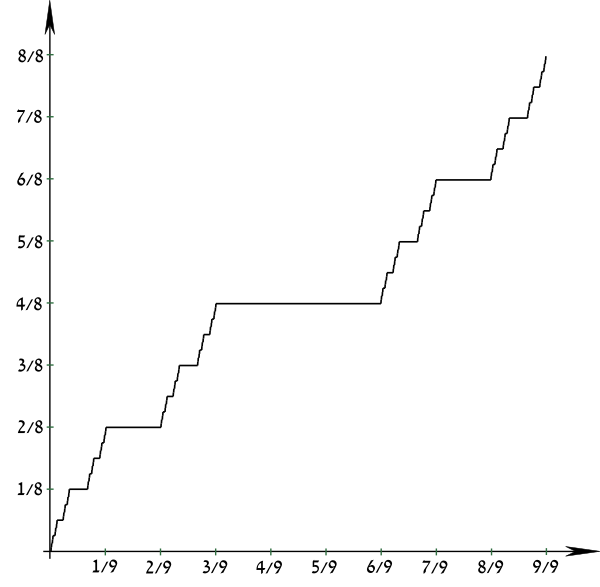
\includegraphics[scale=0.3]{img/devils_staircase.png}
      \caption{Plot} 
      \label{fig:devils_staircase}
    \end{figure}
  \end{definition} 

  \begin{theorem}[Properties of Cantor-Lebesgue Function]
    $\phi$ is a nondecreasing, continuous function s.t. $\phi^\prime (x) = 0$ for all $x \in O$ and $m(O) = 1$. 
  \end{theorem}
  \begin{proof}
    Listed. 
    \begin{enumerate}
      \item \textit{Increasing}. $\phi$ is increasing on each $O_k$, and so on $O$. Then, it is also increasing on $C$ by definition. 
      \item \textit{Continuity}. If $x \in C$, it lies between 2 intervals of $O_k$ for any $k$. The difference in function values between 2 neighboring intervals of $O_k$ is $2^{-k}$, so $\phi$ is continuous. 
      \item \textit{Derivative}. The derivative is $0$ because it is constant around an interval. 
    \end{enumerate}
  \end{proof}

  \begin{theorem}[Pathological Strictly Increasing Devil's Staircase][thm:pathological-devils-staircase]
    Define $\psi (x) = \phi(x) + x$. Then, 
    \begin{enumerate}
      \item $\psi$ is continuous and strictly increasing. 
      \item $\psi$ maps $C$ into a set of positive measure. 
      \item $\psi$ maps some subset of $C$ into a nonmeasurable set. 
    \end{enumerate}
  \end{theorem}
  \begin{proof}
    Listed. 
    \begin{enumerate}
      \item Continuity is from sum of continuous functions, and strictly increasing since $\phi$ is nondecreasing and $x$ is strictly increasing. 
      \item We know that $\psi([0, 1]) = [0, 2]$ and $m(\psi(O))= 1$, where for each interval $I_j \subset O$, $m(\psi(I_j)) = \ell(I_j)$. Therefore, $m(\psi(C)) = 1$. 
      \item Since $\psi$ is strictly increasing, there exists a continuous inverse $\psi^{-1}$. Find $Z \subset \psi(C)$ that is nonmeasurable, which we can do from the previous theorem. Then, there exists $E \subset C$ s.t. $\psi(E) = Z$, and $E$ is not Borel since if it were, then $Z$ would be Borel, too. 
    \end{enumerate}
  \end{proof}

\subsection{Signed Measures}

  \begin{lemma}[Sums and Positive Multiples of Measures are Measures]
    If $\mu_1$ and $\mu_2$ are two measures defined on the same measurable space $(X, \mathcal{M})$, then for $\alpha, \beta > 0$, the following is a measure as well. 
    \begin{equation}
      \mu_3 (E) = \alpha \cdot \mu_1 (E) + \beta \cdot \mu_2 (E)
    \end{equation}
  \end{lemma}
  \begin{proof}
    
  \end{proof}

  Note that we can't always define differences of such measures 
  \begin{equation}
    \nu(E) = \mu_1 (E) - \mu_2 (E)
  \end{equation}
  since $\nu$ may not always be nonnegative. Furthermore, it may not even be defined if $\mu_1 (E) - \mu_2 (E) = \infty - \infty$. 

  \begin{definition}[Signed Measure]
    A \textbf{signed measure} $\nu$ on the measurable space $(X, \mathcal{M})$ is a function $\nu: \mathcal{M} \to [-\infty, +\infty]$ satisfying 
    \begin{enumerate}
      \item \textit{Well-Defined}. $\nu$ assumes at most one of the values $+\infty, -\infty$. 
      \item \textit{Null Empty Set}. $\nu(\emptyset) = 0$ 
      \item \textit{Countable Additivity}. For any countable collection $\{E_k\}_{k=1}^\infty$ of disjoint measurable sets, 
        \begin{equation}
          \nu \bigg( \bigcup_{k=1}^\infty E_k \bigg) = \sum_{k=1}^\infty \nu(E_k)
        \end{equation}
        where the series $\sum_{k} \nu(E_k)$ converges absolutely if $\nu \big( \cup_{k} E_k \big)$ is finite. 
    \end{enumerate}
  \end{definition} 

  \begin{definition}[Positive, Negative, Null Sets]
    Let $\nu$ be a signed measure on $(X, \mathcal{M})$ and $A \in \mathcal{M}$. 
    \begin{enumerate}
      \item $A$ is \textbf{positive} w.r.t. $\nu$ if for all measurable $E \subset A$, $\nu(E) \geq 0$. 
      \item $A$ is \textbf{negative} w.r.t. $\nu$ if for all measurable $E \subset B$, $\nu(E) \leq 0$. 
      \item $A$ is \textbf{null} w.r.t. $\nu$ if for all measurable $E \subset B$, $\nu(E) = 0$.\footnote{By monotoncity of measure, a set is null if and only if it has measure $0$.}
    \end{enumerate}
  \end{definition}

  \begin{lemma}[Hahn's Lemma]
    Let $\nu$ be a signed measure on $(X, \mathcal{M})$ and $E$ a measurable set for which $0 < \nu(E) < +\infty$. Then, there is a measurable subset $A \subset E$ that is positive and of positive measure. 
  \end{lemma}

  \begin{theorem}[Hahn Decomposition Theorem]
    Let $\nu$ be a signed measure on the measurable space $(X, \mathcal{M})$. Then, there is a positive set $A$ and a negative set $B$, both with respect to $\nu$, for which 
    \begin{equation}
      X = A \sqcup B
    \end{equation}
    That is, we can always decompose $X$ into a positive and negative measure parts, and this is called the \textbf{Hahn decomposition} of $X$ w.r.t. $\nu$.\footnote{Note that this may not be unique, since if $A \cup B$ is a Hahn decomposition, then by excising a null set $E$ from $A$ and adding to $B$, $(A \setminus E) \cup (B \cup E)$ is also a Hahn decomposition.} 
  \end{theorem}

  Therefore, the measure of $\nu^+ (E) = \nu (E \cap A)$ and $\nu^- (E) = -\nu(E \cap B)$. This decomposition is nice since we know that the positive parts and the negative parts are ``nicely separated.'' Let's formalize this notion. 

  \begin{definition}[Mutually Singular Measures]
    Two measures $\nu_1, \nu_2$ are said to be \textbf{mutually singular}, denoted $\nu_1 \perp \nu_2$, if $X = A \cup B$ with $\nu_1 (A) = \nu_2 (B) = 0$. 
  \end{definition}

  \begin{theorem}[Jordan Decomposition Theorem]
    Let $\nu$ be a signed measure on the measurable space $(X, \mathcal{M})$. Then, there is a unique pair of mutually singular measures $\nu^+, \nu^-$ on $(X, \mathcal{M})$ for which 
    \begin{equation}
      \nu = \nu^+ - \nu^- 
    \end{equation}
    called the \textbf{Jordan decomposition}, with $\nu^+, \nu^-$ called the positive and negative parts of $\nu$. Since $\nu$ assumes at most one of the values $\pm \infty$, either $\nu^+, \nu^-$ must be finite. 
  \end{theorem}
  \begin{proof}
    We have already proven the first part as 
    \begin{equation}
      \nu^+ (E) = \nu (E \cap A), \quad \nu^- (E) = -\nu(E \cap B)
    \end{equation}
  \end{proof}

  \begin{example}[]
    Let $f: \mathbb{R} \to \mathbb{R}$ be a function that is Lebesgue integrable over $\mathbb{R}$, and define 
    \begin{equation}
      \nu(E) \coloneqq \int_E f \,dm
    \end{equation}
    Then, from the countable additivity of integration, $\nu$ is a signed measure on the measurable space $(\mathbb{R}, \mathcal{L})$. Define 
    \begin{equation}
      A = \{x \in \mathbb{R} \mid f(x) \geq 0 \}, \quad B = \{x \in \mathbb{R} \mid f(x) < 0 \}
    \end{equation}
    and 
    \begin{equation}
      \nu^+ (E) = \int_{A \cap E} f \,dm, \quad \nu^- (E) = - \int_{B \cap E} f \,dm
    \end{equation}
    Then, $A, B$ is a Hahn decomposition of $\mathbb{R}$ w.r.t. the signed measure $\nu$. Moreover, $v = v^+ = v^-$ is a Jordan decomposition of $\nu$. 
  \end{example}

\subsection{Sigma Finite Measures}

  \begin{definition}[Finite, $\sigma$-Finite Measures and Measurable Sets]
    Let $(X, \mathcal{M}, \mu)$ be a measure space. 
    \begin{enumerate}
      \item The measure $\mu$ is \textbf{finite} if $\mu(X) < +\infty$. 
      \item The measure $\mu$ is \textbf{$\sigma$-finite} if $X$ is the union of a countable collection of measurable sets, each of which has finite measure. 
    \end{enumerate}
    Let $E$ be a measurable set. 
    \begin{enumerate}
      \item $E$ is of \textbf{finite measure} if $\mu(E) < +\infty$. 
      \item $E$ is \textbf{$\sigma$-finite} if $E$ is the union of a countable collection of measurable sets, each of which has finite measure. 
    \end{enumerate}
    Finiteness implies $\sigma$-finiteness. 
  \end{definition}

  \begin{example}
    Listed. 
    \begin{enumerate}
      \item The Lebesgue measure on $[0, 1]$ is a finite measure. 
      \item The Lebesgue measure on $\mathbb{R}$ is a $\sigma$-finite measure. 
      \item The counting measure on an uncountable set is not $\sigma$-finite.  
    \end{enumerate}
  \end{example}

\subsection{Measures on the Real Line}

  We will see that 
  \begin{enumerate}
    \item Borel $\implies$ measurable. 
    \item Countable $\implies$ measure 0 $\implies$ measurable. 
  \end{enumerate} 
  But none of the reverse implications follow. For example, the Cantor set is measure 0 but uncountable. There is a subset of Cantor set that is measurable but not Borel. The Vitali set is not even measurable at all. 

  We have seen that there are some common sets that are not Jordan measurable, but a bigger problem is that countable unions and intersections aren't. 

  \begin{example}[Countable Union/Intersection of Jordan Measurable Sets are Not J.M.]
    We show a few counterexamples. 
    \begin{enumerate}
      \item \textit{Countable Union}. Take $\mathbb{N} = \{n\}_{n=1}^\infty$. Each point $n$ has Jordan measure $0$, but their union is unbounded so it isn't Jordan measurable. 

      \item \textit{Bounded Countable Union}. Maybe we can fix this by considering bounded unions. But consider $E = \mathbb{Q} \cap [0, 1]$. By density of rationals, 
      \begin{equation}
        m_\ast (E) = 0 \neq 1 = m^\ast (E)
      \end{equation}
        
      \item \textit{Intersection}. Consider the Cantor set $C$, which is bounded, but again 
      \begin{equation}
        m_\ast (C) = 0 \neq 1 = m^\ast (C)
      \end{equation}
    \end{enumerate}
  \end{example}

  This motivates the definition of a $\sigma$-algebra. 

  \begin{definition}[$\sigma$-Algebra]
    A \textbf{$\boldsymbol{\sigma}$-algebra} on a set $X$ is a collection of subsets of $X$ satisfying the following: 
    \begin{enumerate}
      \item \textit{Contains Empty and Full Set}. $\emptyset, X \in \mathcal{A}$. 
      \item \textit{Closed Under Countable Unions}. $A_n \in \mathcal{A}$ for all $n \in \mathbb{N}$ implies $\bigcup_n A_n \in \mathcal{A}$. 
      \item \textit{Closed Under Complements}. $A \in \mathcal{A} \implies A^c \in \mathcal{A}$. 
      \item \textit{Closed Under Countable Intersections}.\footnote{This is actually a consequence of the previous properties. We can utilize the fact that $\cap_{k=1}^\infty A_k = X \setminus \cup_{k=1}^\infty A_k^c$ } $A_n \in \mathcal{A}$ for all $n \in \mathbb{N}$ implies $\bigcap_n A_n \in \mathcal{A}$. 
    \end{enumerate}
  \end{definition}

  In some applications, we can just ignore some of these sets as ``pathological.'' But for Riemann integrability, we are integrating over Jordan measurable sets (closed and bounded intervals). It turns out that it is really important that we can \textit{at least} guarantee that countable unions and intersections of Jordan measurable sets are measurable. If we don't, then not even uniform convergence---an extremely strong property---can preserve continuity, differentiability, and integrability of a sequence of functions. 

  A $\sigma$-algebra is similar to the topology $\mathscr{T}$ of topological space. Both $\mathcal{A}$ and $\mathscr{T}$ require $\emptyset$ and $X$ to be in it. The three differences are that (i) $\mathscr{T}$ does not allow compelmentation, (ii) $\mathscr{T}$ allows any (even uncountable) union of sets (condition is strengthened), and (iii) $\mathscr{T}$ allows only finite intersection of sets (condition is weakened). Now in order to construct $\sigma$-algebras, the following theorems are useful since they allow us to construct $\sigma$-algebras from other $\sigma$-algebras. It turns out that the intersection of $\sigma$-algebras is a $\sigma$-algebra, but not for unions. 

  \begin{theorem}
    Let $\{\mathcal{A}_k\}$ be a family of $\sigma$-algebras of $X$. Then, $\cap \mathcal{A}_k$ is also a $\sigma$-algebra of $X$. 
  \end{theorem}
  \begin{proof}
    Clearly, $\emptyset, X$ is in $\cap \mathcal{A}_k$. To prove complementation, 
    \begin{equation}
      A \in \bigcap \mathcal{A}_k \implies A \in \mathcal{A}_k \; \forall k \implies A^c \in A_k \; \forall k \implies A^c \in \bigcap \mathcal{A}_k
    \end{equation}
    To prove countable union, let $\{A_j\}_{j \in J}$ be some countable family of subsets in $\cap \mathcal{A}_k$. Then, 
    \begin{equation}
      A_j \in \bigcap \mathcal{A}_k \; \forall j \in J \implies A_j \in \mathcal{A}_k \; \forall k \forall j \implies \bigcup A_j \in \mathcal{A}_k \; \forall k \implies \bigcup A_j \in \bigcap \mathcal{A}_k
    \end{equation}
  \end{proof}

  This allows us to easily prove the following theorem, which just establishes the existence of $\sigma$-algebras. 

  \begin{theorem}
    Let $F \subset 2^X$ be a collection of subsets of $X$. Then there exists a unique smallest $\sigma$-algebra $\sigma(F)$ containing $F$. $\sigma(F)$ is called the $\sigma$-algebra \textbf{generated} by $F$. 
  \end{theorem}
  \begin{proof}
    Let us denote $\mathcal{M}$ as the set of all possible $\sigma$-algebras $\mathcal{B}$ of $X$. $\mathcal{M}$ is nonempty since it contains $2^X$. Then, the intersection 
    \begin{equation}
      \bigcap_{\mathcal{B} \in \mathcal{M}} \mathcal{B}
    \end{equation}
    is the unique smallest $\sigma$-algebra. 
  \end{proof}


  Therefore, we would like the collection of our measurable sets to be a $\sigma$-algebra. To do this, we tinker around with the definition of the Jordan measure. Note that by definition, the Jordan outer measure can be equivalently written as 
  \begin{align}
    m^\ast (S) & \coloneqq \inf \{ m(E) \mid S \subset E, E \text{ elementary} \} \\ 
               & = \inf \bigg\{ \sum_{i=1}^k |B_i| \;\bigg|\; S \subset \bigcup_{i=1}^k B_i, B_i \text{ boxes}, k \in \mathbb{N} \bigg\}
  \end{align}
  Note that the \textit{finite} number of boxes $k$ are allowed to vary over all naturals. To define the Lebesgue measure, we change the finite to countable.

  \begin{definition}[Lebesgue Outer Measure]
    Given any set $E \subset \mathbb{R}^n$, the \textbf{Lebesgue outer measure} is a map 
    \begin{equation}
      m^\ast : 2^{\mathbb{R}^n} \to [0, +\infty], \qquad m^\ast (E) = \inf  \left\{ \sum_{k=1}^\infty |B_k| \; \bigg| \; E \subset \bigcup_{k=1}^\infty B_k \right\} 
    \end{equation}
  \end{definition} 

  It's a hard definition, but a natural one, since we're taking all these boxes and trying to make them as snug as possible to define the outer measure of an arbitrary set. We first first check that this is indeed a generalization of Jordan measure, in the sense that if $E$ is Jordan measurable, then its Lebesgue outer measure is the same as its Jordan measure. 

  \begin{theorem}[Lebesgue Outer Measure Coincides with Interval Length]
    $m^\ast$ satisfies the property that for any interval $I \subset \mathbb{R}$, $m^\ast (I) = |I|$. 
  \end{theorem}
  \begin{proof}
    Let's first consider the case when $I$ is closed. Let $I = [a, b]$. Then, we know from definition that 
    \begin{equation}
      m^\ast (I) \coloneqq \inf \bigg\{ \sum_{k=1}^\infty |I_k| \;\bigg|\; I \subset \bigcup_{k=1}^\infty I_k\bigg\}
    \end{equation}
    where $I_k = [a_n, b_n]$. We wish to show that the above quantity equals $b - a$. 
    \begin{enumerate}
      \item $m^\ast (I) \leq b - a$. This is pretty easy since we can just set the cover to consist of the single interval $I$, and since $m^\ast (I)$ must be the infimum of it, then we must have $m^\ast(I) \leq b - a$. A technicality is that we must strictly use countable covers, but in this case, we can just fix $\epsilon > 0$ and see 
      \begin{equation}
        I_1 = [a, b], \qquad I_k = [b - \frac{\epsilon}{2^k}, b + \frac{\epsilon}{2^k}]
      \end{equation}
      In this case the sums of lengths of all $I_2, \ldots$ is $\epsilon/2 < \epsilon$, and so 
      \begin{equation}
        I_k \leq b - a + \epsilon \qquad \forall \epsilon > 0 
      \end{equation}

      \item Proving $m^\ast (I) \geq b - a$ is harder. In here, we use the ``$\epsilon$ of room'' trick. Take any $\epsilon > 0$. Then there exists a cover $\{I_k\}_k$ s.t. 
      \begin{equation}
        m^\ast(I) = \epsilon \geq \sum_{k=1}^\infty |I_k| = \sum_{k=1}^\infty b_k - a_k
      \end{equation}
      All we wish to show that the RHS $\geq b - a$, but we can't really manipulate the infinite sum. This is where we use the fact that $[a, b]$ is compact\footnote{since it's closed and bounded}, and so we can take a finite subcover $\{I_{k_j}\}_{j=1}^n$. Therefore, 
      \begin{equation}
        m^\ast (I) + \epsilon  \geq \sum_{j=1}^n b_{k_j} - a_{k_j} 
      \end{equation}
      Now we can rearrange this: set the $a_{k_j}$'s to be increasing, and for simplicity let's reindex them to $a_j, b_j$. Then, it must be the case that $a_1 < a$. 
      \begin{enumerate}
        \item Consider $(a_1, b_1)$. If $b_1 > b$, we are done. 
        \item Otherwise, $b_1 \in (a_2, b_2)$. If $b_2 > b$, then 
        \begin{equation}
          b_2 - a_2 + b_1 - a_1 \geq b_2 - a_1 > b - a
        \end{equation}
        \item If not, then we keep going until we get to $(a_n, b_n)$. If $b_n > b$, then 
          \begin{equation}
            b_n - a_n + b_{n-1} - a_{n-1} + \ldots + b_1 - a_1 \geq b_n - a_1  > b - a
          \end{equation}
      \end{enumerate}
    \end{enumerate}
  \end{proof}

  The proof may be a bit unfamiliar since we have used two tricks. 
  \begin{enumerate}
    \item \textit{Geometric Sequence of $\epsilon$ Trick}. To account for countable collections, we set $\epsilon$ to be decreasing geometrically so that the series converges to $\epsilon$. 
    \begin{equation}
      \epsilon = \sum_{n=1}^\infty \frac{\epsilon}{2^n}
    \end{equation}

    \item \textit{$\epsilon$ of Room Trick}. This trick is used often when you need an opposite inequality that isn't as obvious, and it can only be used for inequalities involving a supremum or infimum. 
    \begin{equation}
      \inf\{S\} \geq x
    \end{equation}

    By using the definition of sup/inf as the \textit{least} upper/lower bound, we can scooch over by an $\epsilon$ to find an element in $s \in S$ that does satisfy the inequality 
    \begin{equation}
      \inf\{S\} + \epsilon > s \geq x
    \end{equation}
    and since $\epsilon$ was arbitrary, we are done. 
  \end{enumerate}

  It is clear that the Lebesgue outer measure is always less than the Jordan outer measure. 
  \begin{equation}
    m^\ast (E) \leq m^{(J), \ast} (E) 
  \end{equation}
  When are these different? 

  \begin{example}[Lebesgue Outer Measure Much Smaller than Jordan Outer Measure]
    Consider $\mathbb{Q}$. 
    \begin{enumerate}
      \item The Jordan outer measure is $+\infty$ since it is unbounded. 
      \item However, any countable set of $\mathbb{R}$ has Lebesgue outer measure $0$. Just enumerate $E = \{x_1, \ldots \}$. Then, we set $I_k = \big( x_k - \frac{\epsilon}{2^k}, x_k + \frac{\epsilon}{2^k} \big)$. Then, 
      \begin{equation}
        \sum_{k=1}^\infty \ell(I_k) = \epsilon
      \end{equation}
    \end{enumerate}
  \end{example}

  What about the inner measure? It turns out that we don't get much if we replace the finite to countable in the Jordan inner measure. 

  \begin{lemma}[Axiomatic Properties of Lebesgue Outer Measure]
    The Lebesgue outer measure satisfies the following. 
    \begin{enumerate}
      \item \textit{Null Empty Set}. $m^\ast(\emptyset) = 0$. 
      \item \textit{Monotonicity}. Given sets $E \subset F \subset \mathbb{R}^n$, we have 
      \begin{equation}
        m^\ast (E) \leq m^\ast (F)
      \end{equation}
    \item \textit{Countable Subadditivity}. For any countable collection of subsets $\{E_k\}$ of $\mathbb{R}^d$, 
      \begin{equation}
        m^\ast \bigg( \bigcup_n E_n \bigg) \leq \sum_{n} m^\ast (E_n) 
      \end{equation}
    \end{enumerate}
  \end{lemma}
  \begin{proof}
    The first two properties are trivial. For the third, let's start by writing out the definition for the outer measure for each $E_n$. 
    \begin{equation}
      m^\ast (E_n) \coloneqq \inf \bigg\{ \sum_{k=1}^\infty |B_k^{(n)}| \;\bigg|\; E_n \subset \bigcup_{k=1}^\infty B_k^{(n)}, B_k^{(n)} \text{ boxes} \bigg\}
    \end{equation}
    Somehow, we want to sum these values over all $n$ and prove that this is greater than the measure of the union. The first realization should be that for a fixed cover $\{B_k^{(n)}\}_k$ of $E_n$, the collection 
    \begin{equation}
      \{B_k^{(n)}\}_{n, k} \text{ covers } \bigcup_{n} E_n
    \end{equation} 
    This gives us a clue as to comparing the collection of covers of each $E_n$, with the cover of $\cup E_n$. There is no straightforward way to do this,\footnote{On one side, we have the sum of a countable number of infimums of some sets, and on the other hand, we have the infimum of the unions of all of these sets.} so we want to try and \textit{fix} these collections. We can do this with the $\epsilon$ of room trick. For each $E_n$, we can find a cover $\{B_k^{(n)}\}_k$ s.t. 
    \begin{equation}
      m^\ast (E_n) + \frac{\epsilon}{2^n} \geq \sum_{k=1}^\infty |B_k^{(n)}| 
    \end{equation}
    Then, we can take the infinite sum. 
    \begin{equation}
      \sum_{n=1}^\infty \bigg( m^\ast (E_n) + \frac{\epsilon}{2^n} \bigg) \geq \sum_{n=1}^\infty \sum_{k=1}^\infty |B_k^{(n)}| \geq m^\ast \bigg( \bigcup_n E_n \bigg)
    \end{equation} 
    where the final inequality follows from the fact that $\{B_k^{(n)}\}_{n, k}$ is a cover of $\cup_n E_n$, and so it must be greater than the infimum of all possible covers. All monotonic series converge in $[0, +\infty]$, so we can ``take out'' the $\epsilon$ term to get 
    \begin{equation}
      \epsilon + \sum_{n=1}^\infty m^\ast (E_n) \geq m^\ast \bigg( \bigcup_n E_n \bigg)
    \end{equation}
    which holds for all $\epsilon > 0$, and so we are done. 
  \end{proof}

  \begin{theorem}[Translation Invariance of Lebesgue Outer Measure]
    $m^\ast$ is translation invariant. That is, for any $E \subset \mathbb{R}^n$, 
    \begin{equation}
      m^\ast (E) = m^\ast (E + a), \qquad E + a \coloneqq \{x + a \in \mathbb{R}^n \mid a \in E \}
    \end{equation}
  \end{theorem}
  \begin{proof}
    This is straightforward and requires no tricks. Note that 
    \begin{equation}
      \{B_k\} \text{ is a countable cover of } E \iff \{B_k + a\} \text{ is a countable cover of } E + a
    \end{equation}
    It is also clear that 
    \begin{equation}
      |B| = |B + a| 
    \end{equation}
    for any box $B \subset \mathbb{R}^n$, so the sets of sizes that we are taking the infimum over is exactly the same between the two. 
  \end{proof}

  The final property claims that we can always drop an outer-measure $0$ set and it won't affect the outer measure of the original set. Therefore, when talking about measurability of intervals, we don't have to worry about endpoints, or even whether it is missing a countable number of elements from it! 

  \begin{lemma}[Sets of Outer Measure 0 Doesn't Affect Outer Measure]
    Suppose $m^\ast (E) = 0$ and $A$ is any set. 
    \begin{enumerate}
      \item Adding a set of outer measure $0$ doesn't affect the outer measure. 
        \begin{equation}
          m^\ast (A \cup E) = m^\ast (A)
        \end{equation}
      \item Excising a set of outer measure $0$ doesn't affect the outer measure. 
        \begin{equation}
          m^\ast (A \setminus E) = m^\ast (A)
        \end{equation}
    \end{enumerate}
  \end{lemma}
  \begin{proof}
    Listed. 
    \begin{enumerate}
      \item We have 
        \begin{equation}
          m^\ast (A \cup E) = \underbrace{m^\ast \big( (A \cup E) \cap E \big)}_{=0} + m^\ast \underbrace{\big( (A \cup E) \cap E^c \big)}_{\subset A} \leq m^\ast (A) \leq m^\ast (A)
        \end{equation}
        But $A \cup E \supset A$, so $m^\ast (A \cup E) = m^\ast (A)$. 
      \item Note that $m^\ast (A \setminus E) \leq m^\ast (A)$ by monotonicity. Also, by subadditivity
        \begin{equation}
          m^\ast (A) \leq m^\ast (A \setminus E) + \underbrace{m^\ast (E)}_{=0} = m^\ast (A \setminus E)
        \end{equation}
    \end{enumerate}
  \end{proof} 

  \begin{lemma}[Finite Additivity for Outer Measure][lem:finite-additivity-for-outer-measure]
    Let $A$ and $B$ be bounded sets for which there is an $\alpha > 0$ such that $|a - b| \geq \alpha$ for all $a \in A$, $b \in B$. Prove that $m^{\ast}(A \cup B) = m^{\ast}(A) + m^{\ast}(B)$.\footnote{This is a slightly weaker version of Tao Lemma 1.2.5. }
  \end{lemma}
  \begin{proof}
    The ideas is that if we have some cover $\{I_k\}$ of $A \cup B$, then either $I_k$ only intersects $A$ (and thus contributes to covering $A$ only), only intersects $B$, or intersects both $A$ and $B$ (and thus also covers some non-essential interval of length $\alpha$). Since $A, B$ are bounded, $m^\ast (A), m^\ast (B) < +\infty$. We wish to show that 
    \begin{equation}
      m^\ast (A) + m^\ast (B) \leq m^\ast (A \cup B) \iff m^\ast (A) + m^\ast (B) < m^\ast (A \cup B) + \epsilon \quad \forall \epsilon > 0
    \end{equation}
    By setting $\epsilon = \frac{\alpha}{2}$, we can force the covering to consist of intervals that can intersect only $A$ and $B$, but not both. If such an interval $I$ did, then it would contain a set of measure $\geq \alpha$, so 
    \begin{equation}
      m(I) \geq \alpha \implies \sum_{k=1}^\infty \ell(I_k) \geq m(A \cup B) + \alpha 
    \end{equation}
    Therefore, we can partition all such covers to cover $A$ and $B$, respectively, meaning 
    \begin{equation}
      m^\ast (A \cup B) + \frac{\alpha}{2} > \sum \ell(I_k) + \sum \ell(I_k) \geq m^\ast (A) + m^\ast(B)
    \end{equation}
  \end{proof}
  
  Therefore we can invoke this in special cases where \hyperref[real-ex:compact-closed-dist]{one set may be compact and another may be closed}.


  The next step is to take the outer measure and define \textit{Lebesgue measurable} sets. The problem is that---unlike the Jordan measure---we don't have the inner measure to work with. This turns out to be not much of a problem, since through \textit{Littlewood's first principle}\footnote{One of the major themes in measure theory, where we say that measurable sets are well-approximated by open and closed sets.}, we can define measurability as being well-approximated by an open set. 
  
  \begin{definition}[Lebesgue Measurable Set]
    A set $E \subset \mathbb{R}^d$ is \textbf{Lebesgue measurable} if for every set $A \subset \mathbb{R}^n$, 
    \begin{equation}
      m^\ast (A) = m^\ast (A \cap E) + m^\ast (A \cap E^c)
    \end{equation}
    which is known as \textit{Carathéodory's criterion}. Colloquially, no matter how nasty a subset $A$ is, $E$ should be nice enough that we can cut $E$ into two pieces $C$ and $D$.
  \end{definition}

  Note that due to countable subadditivity, we are guaranteed to have $\leq$. Therefore, it suffices to prove only for $\geq$. The sets with which this inequality is strict is not measurable, and the measurable sets specifically satisfy equality for countable sets. So what kind of sets are measurable? 

  \begin{example}[Outer Measure $0$ Sets are Lebesgue Measurable]
    For any outer measure $m^\ast$ on $X$, $E \subset X$ with $m^\ast (E) = 0$  implies that $E$ is $m^\ast$-measurable. Take any $A$. Then $(A \cap E) \subset E$ and $(A \cap E^c) \subset A$. So by monotonicity, 
    \begin{equation}
      m^\ast(A \cap E) + m^\ast (A \cap E^c) \leq m^\ast(E) + m^\ast(A) = m^\ast (A)
    \end{equation}
    and this by definition means that $E$ is measurable. 
  \end{example}

  We could continue with more examples, but our main priority is to show that this family of Lebesgue measurable sets is indeed a $\sigma$-algebra, and it covers much more than Jordan measurable sets. The path to prove that countable unions are measurable is a long one, and we'll a lot of lemmas. 

  \begin{lemma}[Complements of Measurable Sets are Measurable]
    If $E$ is measurable, then so is $E^c$. 
  \end{lemma}
  \begin{proof}
    The definition is symmetric in both $E$ and $E^c$. 
  \end{proof}

  Using unions and complements, we can prove that intersections and set differences of measurable sets are measurable.  

  \begin{lemma}[Finite Intersections of Measurable Sets are Measurable]
    If $E_1, \ldots, E_n$ is measurable, then so is $\cap_{k=1}^n E_k$. 
  \end{lemma}
  \begin{proof}
    By induction, it suffices to prove for $n = 2$. We have 
    \begin{equation}
      E_1 \cap E_2 = (E_1^c \cup E_2^c)^c
    \end{equation}
  \end{proof}

  \begin{lemma}[Set Differences of Measurable Sets are Measurable]
    If $E_1, E_2$ is measurable, then so is $E_1 \setminus E_2$. 
  \end{lemma}
  \begin{proof}
    We have 
    \begin{equation}
      E_1 \setminus E_2 = E_1 \cap E_2^c
    \end{equation}
  \end{proof}

  \begin{lemma}[Excision Property]
    If $E \subset \mathbb{R}^n$ is measurable with $m^\ast (E) < +\infty$, and $E \subset F$ for arbitrary set $F$, then 
    \begin{equation}
      m^\ast (F \setminus E) = m^\ast(F) - m^\ast(E)
    \end{equation}
  \end{lemma}
  \begin{proof}
    By measurability of $E$, we can see 
    \begin{align}
      m^\ast (F) & = m^\ast (F \cap E) + m^\ast (F \cap E^c) \\
                 & = m^\ast (E) + m^\ast (F \setminus E)
    \end{align}
  \end{proof}

  This excision property combined with the fact that outer measure 0 sets are always measurable gives us the property of \textit{completeness}.\footnote{Nothing to do with completeness in the sense of real numbers or metric spaces.} That is, given measurable sets $A \subset B \subset C$ with $m^\ast(A) = m^\ast (C)$, $B$ must be measurable. This basically says that if you a set that is squeezed in between two measurable sets of equal measure, then the middle set will also be measurable. 

  \begin{lemma}[Finite Unions are Measurable]
    A finite union of measurable sets is measurable. 
  \end{lemma}
  \begin{proof}
    This proof is basically applying set theory laws, and there's not much more to that. It suffices to prove for $E_1, E_2$, and the rest follows by induction. Fix any $A$. Then 
    \begin{align}
      m^\ast (A) & = m^\ast (A \cap E_1) + m^\ast (A \cap E_1^c) \\ 
                   & = m^\ast (A \cap E_1) + m^\ast \big(A \cap E_1^c \cap E_2 \big) + m^\ast \big((A \cap E_1^c) \cap E_2^c \big)
    \end{align}
    Now we apply the identity $(A \cap E_1^c) \cap E_2^c = A \cap (E_1 \cup E_2)^c$, so the third term can be changed 
    \begin{equation}
      = m^\ast (A \cap E_1) + m^\ast \big((A \cap E_1^c) \cap E_2 \big) + m^\ast \big( A \cap (E_1 \cup E_2)^c \big)
    \end{equation}
    Then we apply the identity $(A \cap E_1) \cup (A \cap E_1^c \cap E_2) = A \cap (E_1 \cup E_2)$, so we can apply finite subadditivity on the first two terms to get 
    \begin{equation}
      \geq m^\ast (A \cap (E_1 \cup E_2)) + m^\ast \big( A \cap (E_1 \cup E_2)^c \big)
    \end{equation}
    which proves that $E_1 \cup E_2$ is measurable. 
  \end{proof} 

  So we have proved that the set of all measurable sets is closed under finite unions. By definition it works for finite intersections. This makes it into an \textit{algebra}, but we want to upgrade this to a $\sigma$-algebra by proving closure under \textit{countable} unions. We first prove a lemma. 

  \begin{lemma}[Finite Additivity of Outer Measure for Measurable Sets]
    Suppose $A$ is any set, $\{E_k\}_{k=1}^n$ disjoint and measurable.\footnote{Note that while outer measure isn't finitely additive for arbitrary sets, it is finitely additive for \textit{measurable} sets.} Then, 
    \begin{equation}
      m^\ast \bigg( A \cap \Big( \bigcup_{k=1}^n E_k \Big) \bigg) = \sum_{k=1}^n m^\ast (A \cap E_k)
    \end{equation}
    In particular, 
    \begin{equation}
      m^\ast \bigg( \bigcup_{k=1}^n E_k \bigg) = \sum_{k=1}^n m^\ast (E_k)
    \end{equation}
  \end{lemma}
  \begin{proof}
    It should be clear that we prove by induction, and intuitively, this disjointness should be essential for canceling out some measure terms. $n = 1$ is trivial. This takes a bit of fiddling around with where we should start, but if we just look at the LHS, we can try and use Carathéodory, by setting the arbitrary set to be $B = A \cap (\cup_{k} E_k)$ and  writing $m^\ast (B) = m^\ast(B \cap E_n) + m^\ast(B \cap E_n^c)$. 
    \begin{align}
      m^\ast \bigg( A \cap \Big( \bigcup_{k=1}^n E_k \Big) \bigg) 
        & = m^\ast \Bigg( \bigg( A \cap \Big( \bigcup_{k=1}^n E_k \Big) \bigg) \cap E_n \Bigg) + m^\ast \Bigg( \bigg( A \cap \Big( \bigcup_{k=1}^n E_k \Big) \bigg) \cap E_n^c \Bigg) \\  
        & = m^\ast (A \cap E_n) + m^\ast \bigg( A \cap \Big( \bigcup_{k=1}^{n-1} E_k \Big) \bigg) \\ 
        & = \sum_{k=1}^n m^\ast (A \cap E_k)
    \end{align}
    But note that by disjointness, we have 
    \begin{equation}
      \bigg( A \cap \Big( \bigcup_{k=1}^n E_k \Big) \bigg) \cap E_n = A \cap E_n, \qquad \bigg( A \cap \Big( \bigcup_{k=1}^n E_k \Big) \bigg) \cap E_n^c = A \cap \Big( \bigcup_{k=1}^{n-1} E_k \Big)
    \end{equation}
    by the induction hypothesis. \qed Here is a wrong proof that does an incorrect form of induction. I first assumed that we can just work with a family of two sets $E_1, E_2$, so I started deriving something like this: 
    \begin{align}
      m^\ast(A) & = m^\ast (A \cap (E_1 \cup E_2)) + m^\ast (A \cap (E_1 \cup E_2)^c ) \\ 
                & = m^\ast ((A \cap E_1) \cup (A \cap E_2) + \underbrace{m^\ast ((A \setminus E_1) \cap (A \setminus E_2))}_{\geq 0} \\ 
                & \geq m^\ast ((A \cap E_1) \cup (A \cap E_2)) 
    \end{align}
    Note that the $E_k$'s being disjoint means that they are \textit{pairwise} disjoint, and so it is \textit{not} sufficient to prove for only $E_1, E_2$. So don't do this. 
  \end{proof}

  \begin{theorem}[Countable Unions are Measurable]
    Suppose $E_1, E_2, \ldots$ are a countable collection of measurable sets. Then, $E = \cup_{j=1}^\infty E_j$ is measurable. 
  \end{theorem}
  \begin{proof}
    They key is to look at disjoint sets. WLOG, one can assume $E_j$ are disjoint. Indeed, we can define new sets
    \begin{equation}
      E_n^\prime \coloneqq E_n \setminus \bigg( \bigcup_{j=1}^{n-1} E_j \bigg) 
    \end{equation}
    that are measurable, with $\cup E_n^\prime = \cup E_n$. Now, fix any set $A$. Define sets $F_n = \cup_{j=1}^n E_j$. Then, $m^\ast (A) = m^\ast (A \cap F_n) + m^\ast (A \cap F_n^c)$. Then, $F_n^c \supset E^c \implies m^\ast (A \cap F_n^c) \geq m^\ast (A \cap E^c)$. Since we have established from the previous lemma that outer measure on disjoint measurable sets satisfies finite additivity, we can write
    \begin{equation}
      m^\ast (A \cap F_n) = m^\ast \bigg( \bigcup_{j=1}^n (A \cap E_j) \bigg) = \sum_{j=1}^n m^\ast (A \cap E_j) 
    \end{equation}
    Then, 
    \begin{equation}
      m^\ast (A) \geq \sum_{j=1}^n m^\ast (A \cap E_j) + m^\ast (A \cap E^c) 
    \end{equation}
    for every $n$, therefore also with $\infty$. But by countable subadditivity of the outer measure, 
    \begin{equation}
      \sum_{j=1}^\infty m^\ast (A \cap E_j) \geq m^\ast (A \cap E)
    \end{equation}
    If follows that $m^\ast (A) \geq m^\ast (A \cap E) + m^\ast (A \cap E^c)$. 
  \end{proof}
  \begin{proof}
    \textit{In class}. We first prove this lemma, which is more general (arbitrary intersections than finite?). Suppose $A$ is any set, $E_j$ disjoint and measurable. Then, 
    \begin{equation}
      \mu^\ast \bigg( A \cap \Big( \bigcup_{j=1}^n E_j \Big) \bigg) = \sum_{j=1}^n \mu^\ast (A \cap E_j)
    \end{equation}
    By induction, $n = 1$ is true. Then, 
    \begin{align}
      \mu^\ast \bigg( A \cap \Big( \bigcup_{j=1}^n E_j \Big) \bigg) 
        & = \mu^\ast \Bigg( \bigg( A \cap \Big( \bigcup_{j=1}^n E_j \Big) \bigg) \cap E_n \Bigg) + \mu^\ast \Bigg( \bigg( A \cap \Big( \bigcup_{j=1}^n E_j \Big) \bigg) \cap E_n^c \Bigg) \\  
        & = \mu^\ast (A \cap E_n) + \mu^\ast \bigg( A \cap \Big( \bigcup_{j=1}^{n-1} E_j \Big) \bigg) \\ & = \sum_{j=1}^n \mu^\ast (A \cap E_j) \end{align}
    by the induction hypothesis. 
    
    They key is to look at disjoint sets. WLOG, one can assume $E_j$ are disjoint. Indeed, we can define new sets 
    \begin{equation}
      E_n^\prime \coloneqq E_n \setminus \bigg( \bigcup_{j=1}^{n-1} E_j \bigg) 
    \end{equation}
    that are measurable, with $\cup E_n^\prime = \cup E_n$. Now, fix any set $A$. Define sets $F_n = \cup_{j=1}^n E_j$. Then, $\mu^\ast (A) = \mu^\ast (A \cap F_n) + \mu^\ast (A \cap F_n^c)$. Then, $F_n^c \supset E^c \implies \mu^\ast (A \cap F_n^c) \geq \mu^\ast (A \cap E^c)$. Through the previous lemma, we have 
    \begin{equation}
      \mu^\ast (A \cap F_n) = \mu^\ast \bigg( \bigcup_{j=1}^n (A \cap E_j) \bigg) = \sum_{j=1}^n \mu^\ast (A \cap E_j) 
    \end{equation}
    Then, 
    \begin{equation}
      \mu^\ast (A) \geq \sum_{j=1}^n \mu^\ast (A \cap E_j) + \mu^\ast (A \cap E^c) 
    \end{equation}
    for every $n$, therefore also with $\infty$. But 
    \begin{equation}
      \sum_{j=1}^\infty \mu^\ast (A \cap E_j) \geq \mu^\ast (A \cap E)
    \end{equation}
    If follows that $\mu^\ast (A) \geq \mu^\ast (A \cap E) + \mu^\ast (A \cap E^c)$. 
  \end{proof}

  \begin{corollary}[Measurable Sets form a $\sigma$-Algebra]
    The set of all Lebesgue measurable sets of $\mathbb{R}^n$ form a $\sigma$-algebra. 
  \end{corollary}
  \begin{proof}
    Listed. 
    \begin{enumerate}
      \item $\emptyset$ is measurable since it has outer measure $0$. 
      \item $\mathbb{R}^n$ is measurable since for any set $A \subset \mathbb{R}^n$, 
      \begin{equation}
        m^\ast (A) = m^\ast(A \cap \mathbb{R}^n) + m^\ast(A \cap (\mathbb{R}^n)^c) = m^\ast(A) 
      \end{equation}
      \item We proved closure under complements. 
      \item We just proved closure under countable union. 
    \end{enumerate}
  \end{proof}

  Now that we have established that Lebesgue measurable sets form a $\sigma$-algebra, let's give some examples. 

  \begin{theorem}[Intervals are Measurable]
    All intervals $I \subset \mathbb{R}$ are measurable. 
  \end{theorem}
  \begin{proof}
    It suffices to prove that every raya $(a, +\infty)$ is measurable, since every interval is a countable union/intersection of such rays. We simply prove using Carathéodory,\footnote{WLOG $a \not\in A$ (since we can take the point out without affecting outer measure). TBD: Do we need this assumption really?} so we wish to show that for any set $A \subset \mathbb{R}$, 
    \begin{equation}
      m^\ast (A) \geq m^\ast (A \cap (a, +\infty)) + m^\ast(A \cap (-\infty, a]) = m^\ast (A^\prime) + m^\ast(A^{\prime\prime})
    \end{equation}
    Again, the fact that we have to prove this nontrivial part of the inequality reminds us of using the $\epsilon$ of room trick. Let us 
    $\{I_k\}_{k=1}^\infty$ is a countable cover of $A$ s.t. 
    \begin{equation}
      m^\ast (A) + \epsilon > \sum_{k=1}^\infty \ell (I_k)
    \end{equation}
    We can take this cover and create two smaller covers, covering $A^\prime$ and $A^{\prime\prime}$. 
    \begin{equation}
      \{I_k^\prime \coloneqq I_k \cap A^\prime\}_k, \qquad \{I_k^{\prime\prime} \coloneqq I_k \cap A^{\prime\prime}\}_k
    \end{equation}
    Since these are valid covers, by definition it must be bounded below by the outer measures. 
    \begin{equation}
      \sum_{k=1}^\infty \ell(I_k^\prime) \geq m^\ast(A^\prime), \qquad \sum_{k=1}^\infty \ell(I_k^{\prime\prime}) \geq m^\ast(A^{\prime\prime})
    \end{equation}
    Now all that remains is to connect the sums together. For each $k$, we have $\ell(I_k) = \ell(I_k^\prime) + \ell(I_k^{\prime\prime})$, and since both series converge in $[0, +\infty]$, we can indeed sum them up as limits to get 
    \begin{equation}
      \sum_{k=1}^\infty \ell(I_k^\prime) + \sum_{k=1}^\infty \ell(I_k^{\prime\prime}) = \sum_{k=1}^\infty \ell(I_k^\prime) + \ell(I_k^{\prime\prime}) = \sum_{k=1}^\infty \ell(I_k) 
    \end{equation}
    Putting the bounds together gives 
    \begin{equation}
      m^\ast (A^\prime) + m^\ast (A^{\prime\prime}) \leq \sum_{k=1}^\infty \ell(I_k^\prime) + \sum_{k=1}^\infty \ell(I_k^{\prime\prime}) = \sum_{k=1}^\infty \ell(I_k)  \leq m^\ast (A) + \epsilon
    \end{equation}
    Since this is true for every $\epsilon > 0$, we are done.  
  \end{proof}

  Note again that this $\epsilon$ of room trick is used so that we can \textit{fix} some open cover that acts as a middle ground between the inequalities that we are trying to prove. Then as we let $\epsilon \to 0$, we are done. 

  \begin{example}[Cantor Set is Measurable]
    Let us define 
    \begin{equation}
      C_0 = [0, 1], \qquad C_1 = [0, 1/3] \cup [2/3, 1], \ldots
    \end{equation}
    Basically, we take our every middle third of each subinterval. So $C_k$ is the union of $2^k$ intervals of size $3^{-k}$. Note that $C_k \subset C_{k-1}$. Now define the \textbf{Cantor set} as 
    \begin{equation}
      C \coloneqq \bigcap_{k=1}^\infty C_k
    \end{equation}
    The Cantor set is measurable since it is a countable intersection of closed sets, which are measurable. 
  \end{example}

  \begin{theorem}[Translations of Sets are Measurable]
    If $E \subset \mathbb{R}^n$ is measurable, then for any $a \in \mathbb{R}^n$, $E + a \coloneqq \{x + a \in \mathbb{R}^n \mid x \in E \}$ is measurable. 
  \end{theorem}
  \begin{proof}
    We again use Carathéodory. Let $A \subset \mathbb{R}^n$ by any set. Then by translation invariance of outer measure, we have 
    \begin{align}
      m^\ast(A) & = m^\ast (A - a) \\ 
                & = m^\ast ((A - a) \cap E) + m^\ast((A - a) \cap E^c) \\ 
                & = m^\ast (A \cap (E + a)) + m^\ast (A \cap (E + x)^c)
    \end{align}
    and so $E + a$ is measurable. 
  \end{proof}

  Now we talk about how Lebesgue measurable sets interact with other common sets, such as open and closed sets in a topology. 

  \begin{theorem}[Regularity Definitions of Lebesgue Measurable Set]
    The following are equivalent in $\mathbb{R}^d$. 
    \begin{enumerate}
      \item $E$ is Lebesgue measurable. 

      \item \textit{Outer Approximately Open}. $\forall \epsilon > 0$, $\exists$ open set $O \supset E$  s.t. $m(O \setminus E) \leq \epsilon$. 

      \item \textit{Inner Approximately Closed}. $\forall \epsilon > 0$, $\exists$ closed set $F \subset E$ s.t. $m^\ast (E \setminus F) < \epsilon$.  

      \item \textit{Outer Exactly $G_\delta$}. $\exists$ a $G_\delta$ set $G$ s.t. $E \subset G$ and $m^\ast (G \setminus E) = 0$. 

      \item \textit{Inner Exactly $F_\sigma$}. $\exists$ a $F_\sigma$ set $F$ s.t. $F \subset E$ and $m^\ast (E \setminus F) = 0$. 
    \end{enumerate}
  \end{theorem}
  \begin{proof}
    Listed. 
    \begin{enumerate}
      \item (2) $\implies$ (1). Then for every $k \in \mathbb{N}$, we can find $O_k \supset E$ s.t. $m^\ast (O_k \setminus E) \leq 1/k$. Define the $G_\delta$ set $G = \cap_{k=1}^\infty O_k$. Then, $(G \setminus E) \subset (O_k \setminus E)$ for all $k \implies m^\ast (G \setminus E) \leq 1/k$ for all $k$. Therefore $m^\ast (G \setminus E) = 0$, and $E = G \setminus (G \setminus E)$ is measurable. 

      \item (1) $\implies$ (2). Assume $m^\ast (E) < +\infty$. Find a cover $\{I_k \}_{k=1}^\infty$ s.t. $\sum_{k=1}^\infty \ell (I_k) \leq m^\ast (E) + \epsilon$ . Call $O = \cup_k I_k$. Since $E$ is measurable, $m^\ast (O \setminus E) = m^\ast (O) - m^\ast (E) \leq \sum_{k=1}^\infty \ell(I_k) - m^\ast (E) \leq \epsilon$ 

      \item (1) $\iff$ (3). Straightforward with argument above.  

      \item (1) $\iff$ (4). Generally, we use the fact that $E$ measurable iff $E^c$ measurable. Find $O \supset E^c$ open, with $m^\ast (O \setminus E^c) \leq \epsilon$. Then $F = O^c$ is closed, $F \subset E$, and $m^\ast (E \setminus F) \leq \epsilon$. 

      \item (1) $\iff$ (5). Same argument as (1) $\iff$ (4). 
    \end{enumerate}
  \end{proof}

  Depending on the context, it is helpful to use one definition over another when proving measurability. Just remember that the Carathéodory definition is the most general, since it doesn't even assume a topology on a space, and that is the definition that we will use by default. 


  This next theorem is a different flavor of Littlewood's first principle. It tells us that we can use a finite union of intervals that ``symmetrically'' approximates measurable sets on the real line. 

  \begin{theorem}[Measurable Sets can be Approximated by Borel Sets]
    Suppose $E$ is measurable, with $m^\ast (E) < +\infty$. For every $\epsilon > 0$, there exists a finite number of intervals $\{I_k\}_{k=1}^n$ s.t. if $O = \cup_{k=1}^n I_k$, then 
    \begin{equation}
      m^\ast (O \setminus E) + m^\ast (E \setminus O) < \epsilon
    \end{equation}
  \end{theorem}
  \begin{proof}
    In here, we use the outer approximately open definition of measurable sets. Since every open set can be written as a countable union of open intervals\footnote{since $\mathbb{R}^n$ is second countable}, we can find a collection of open intervals $\{I_k\}_{k=1}^\infty$ s.t. 
    \begin{align}
      E \subset U \coloneqq \bigcup_{k=1}^\infty I_k, \qquad m^\ast(U \setminus E) \leq \frac{\epsilon}{2}
    \end{align}
    The major thing to do now is to reduce the countable union into a finite union. Note that we can just take any subcollection of the $I_k$'s, and we are guaranteed that their union $O$ will satisfy 
    \begin{equation}
      m^\ast(O \setminus E) \leq m(U \setminus E) \leq \frac{\epsilon}{2}
    \end{equation}
    The problem is that we don't want to take too small of a collection so that the other difference is too big. To do this, we can just select the tail of the series: Find $n$ s.t. $\sum_{k=n+1}^\infty \ell(I_k) \leq \epsilon/2$ where WLOG, $I_k$ are disjoint. Define $O = \cup_{k=1}^n I_k$. Then, we have 
    \begin{align}
      m^\ast (O \setminus E) & \leq m(U \setminus E) \leq \frac{\epsilon}{2} \\ 
      m^\ast (E \setminus O) & \leq m(U \setminus O) \leq \sum_{k=n+1}^\infty \ell(I_k) \leq \frac{\epsilon}{2}
    \end{align}
  \end{proof}

  This symmetry in difference induced me to use the inner approximately closed definition in addition. My idea was to just find a closed set $F$ s.t. $F \subset E \subset U$, but there is no straightforward way of finding one finite collection of intervals $O$. 

  \begin{example}[idk where to put this]
    One should note that in particular, if $E$ is $m^\ast$-measurable and $A$ is any set disjoint from $E$, then we must have 
    \begin{align}
      m^\ast (A \cup E) & = m^\ast ((A \cup E) \cap E) + m^\ast ((A \cup E) \cap E^c) \\ 
                          & = m^\ast (E) + m^\ast (A)
    \end{align}
    which solves a bit of the theorem on measures. 
  \end{example}


  Now by restricting our outer measure to measurable sets, we get our measure. 

  \begin{definition}[Lebesgue Measure]
    The restriction the Lebesgue outer measure $m^\ast$ to the set of all measurable sets $\mathcal{A}$, is called the \textbf{Lebesgue measure} 
    \begin{equation}
      m = m^\ast \big|_{\mathcal{A}}
    \end{equation}
  \end{definition}

  Note that for outer measures, they satisfy both countable subadditivity and finite additivity. With measures, we get the best of both worlds: countable subadditivity. 

  \begin{lemma}[Axiomatic Properties of Lebesgue Measure]
    The Lebesgue measure satisfies the following. 
    \begin{enumerate}
      \item \textit{Null Empty Set}. $m(\emptyset) = 0$. 
      \item \textit{Countable Additivity}. For all countable collections $\{A_k\}_{k=1}^\infty$ of pairwise disjoint subsets $A_k \in \mathcal{A}$\footnote{Remember that we are allowed to take countable unions inside our $\sigma$-algebra, so this makes sense.}, 
      \begin{equation}
        m \bigg( \bigsqcup_{k=1}^\infty A_k \bigg) = \sum_{k=1}^\infty m(A_k)
      \end{equation}
    \end{enumerate}
  \end{lemma}
  \begin{proof}
    Listed. 
    \begin{enumerate}
      \item \textit{Null Empty Set}. Since this is true for outer measure $m^\ast$. 
      \item \textit{Countable Additivity}. $m( \cup E_j) = \sum_j m(E_j)$. $\leq$ is trivial by countable subadditivity of the outer measure. For $\geq$, note that for every $n \in \mathbb{N}$, 
      \begin{equation}
        m \bigg( \bigcup_{j=1}^\infty E_j \bigg) \geq m \bigg( \bigcup_{j=1}^n E_j \bigg) = \sum_{j=1}^n m(E_j) 
      \end{equation}
      where the inequality comes from monotonicity and the equality comes from finite additivity of the outer measure. Now take $n \to \infty$. 
    \end{enumerate}
  \end{proof}

  Unlike the outer measure, monotonicity is not an axiomatic property because of two independent reasons, both sufficient. First, the Lebesgue outer measure suffices. Second, it is actually a direct consequence of the two axiomatic properties.  

  \begin{lemma}[Translation Invariance of Lebesgue Measure]
    The Lebesgue measure is translation invariant. 
  \end{lemma}
  \begin{proof}
    We know that translations of Lebesgue measurable sets are also Lebesgue measurable, and the Lebesgue outer measure is translation invariant. 
  \end{proof}

  Now we provide some ``continuity'' properties of the Lebesgue measure. 

  \begin{theorem}[Continuity From Below]
    If $A_1 \subset A_2 \subset A_3 \subset \ldots$, then 
    \begin{equation}
      m \bigg( \bigcup_{k=1}^\infty A_k \bigg) = \lim_{k \rightarrow \infty} m(A_k)
    \end{equation}
  \end{theorem}
  \begin{proof}
    First, note that the limit on the RHS is defined, since $m(A_k)$ is nondecreasing and so must converge in $[0, +\infty]$. But why does this limit equal to the left hand side? The only property that makes sense to work with is countable additivity, so we should define the disjoint collection 
    \begin{equation}
      B_1 = A_1, \quad B_k = A_k \setminus A_{k-1}
    \end{equation}
    Then, it becomes straightforward 
    \begin{align}
      m \bigg( \bigcup_{k=1}^\infty A_k \bigg) 
        & = m \bigg( \bigcup_{k=1}^\infty B_k \bigg) && \tag{Construction} \\ 
        & = \sum_{k=1}^\infty m(B_k) && \tag{Countable Additivity} \\
        & = \lim_{n \to \infty} \sum_{k=1}^n m(B_k) && \tag{Definition of Series} \\
        & = \lim_{n \to \infty} m \bigg( \bigcup_{k=1}^\infty B_k \bigg) && \tag{Finite Additivity} \\
        & = \lim_{n \to \infty} m(A_k)
    \end{align}
  \end{proof}
  \begin{proof}
    Old proof. We can see that 
    \begin{align}
      m\bigg( \bigcup_{k=1}^\infty A_k \bigg) & = m(A_1) + \sum_{k=2}^\infty m(B_k) \\
      & = m(A_1) + \lim_{k \rightarrow \infty} \sum_{k=2}^\infty m(B_k) \\
      & = \lim_{k \rightarrow \infty} m(A_1 \cup B_2 \cup \ldots B_k)  = \lim_{k \rightarrow \infty} m(A_k) 
    \end{align}
  \end{proof}

  Now a similar theorem, but with a little twist to it. 

  \begin{theorem}[Continuity from Above]
    If $A_1 \supset A_2 \supset A_3 \supset \ldots$, then 
    \begin{equation}
      m\bigg( \bigcap_{k=1}^\infty A_k \bigg) = \lim_{k \rightarrow \infty} m(A_k)
    \end{equation}
    if $m(A_1) < \infty$. 
  \end{theorem}
  \begin{proof}
    First, note that the $m(A_1) < +\infty$ is a necessary condition, since if we take $A_k = [k, \infty)$ on the real number line, then we have $\cap_{k=1}^\infty A_k = \emptyset$, but the limit of the measure is $\infty$. We did not have this problem for continuity from below. 

    Well we can define $B_k = A_k \setminus A_{k+1}$ and write $\cap_{k=1}^\infty A_k = A_1 \setminus \cup_{k=1}^\infty B_k$, which means that 
    \begin{align}
      m\bigg( \bigcap_{k=1}^\infty A_k \bigg) 
        & = m\bigg( A_1 \setminus \bigcup_{k=1}^\infty B_k \bigg) \\
        & = m(A_1) - m\bigg( \bigcup_{k=1}^\infty B_k\bigg) && \tag{Excision} \\
        & = m(A_1) - \sum_{k=1}^\infty m(B_k) && \tag{Countable Additivity} \\
        & = m(A_1) - \lim_{n \rightarrow \infty} \sum_{k=1}^n m(B_k) && \tag{Definition of Series} \\
        & = \lim_{n \rightarrow \infty} \bigg( m(A_1) - \sum_{k=1}^n m(B_k) \bigg) \\
        & = \lim_{n \rightarrow \infty} m \bigg( A_1 \setminus \bigcup_{k=1}^n B_k \bigg) && \tag{Excision} \\ 
        & = \lim_{n \rightarrow \infty} m(A_n) 
    \end{align}
    Now the first line uses the fact that if $A \subset B$, then $m(B \setminus A) + m(A) = m(B)$, and with the further assumption that $m(A) < \infty$, we can subtract on both sides like we do with regular arithmetic. 
  \end{proof}

  We will see two applications of continuity from above. 

  \begin{example}[Cantor Set has Measure 0]
    The Cantor set has measure $0$. We can see that it is the intersection of all $C_k$'s which are nested $C_k \supset C_{k+1}$ and $m(C_0) = m([0, 1]) = 1$. Therefore, by continuity from above, 
    \begin{equation}
      m \bigg( \bigcap_{k=1}^\infty C_k \bigg) = \lim_{k \to \infty} m(C_k) = \lim_{k \to \infty} \frac{2^k}{3^k} = 0 
    \end{equation}

    It is also closed as an intersection of closed sets. It is also uncountable, since we can just do it using a tradic system and see that the Cantor set are all reals with infinite triadic representation of digits $0$ and $2$. Then create a bijection with binary represenation of reals. Here's a new way I learned. Suppose $C$ is countable, so enumerate it: $c_1, c_2, \ldots$. Pick one interval $I_1$ in $C_1$ that doesn't contain $c_1$. Then, pick $I_2 \subset I_1 \cap C_2$ s.t. it doesn't contain $c_2$. Keep going, and we get 
    \begin{equation}
      I_1 \supset I_2 \supset I_3 \supset \ldots 
    \end{equation}
    By nested intervals lemma, these are closed, bounded, and nested, which is nonempty. So we've found a point not in the Cantor set, contradicting the fact that we have enumerated it. 
  \end{example}

  Colloquially, if I give you a bunch of sets so that their total measure if finite, then no point will be hit by an infinite number of the sets. 

  \begin{lemma}[Borel-Cantelli]
    Suppose $\{E_k\}_{k=1}^\infty$ are measurable, with $\sum_{k} m(E_k) < +\infty$. Then, 
    \begin{equation}
      m \big( \limsup E_k \big) \coloneqq m \bigg( \bigcap_{n=1}^\infty \bigcup_{k=n}^\infty E_k \bigg) = 0
    \end{equation}
    That is, all $x \in \mathbb{R}$ belonging to an infinite number of $E_k$, has measure $0$. 
  \end{lemma}
  \begin{proof} 
    Let's consider the $E_k$'s. How can I make a decreasing set of them? We can set 
    \begin{equation}
      B_n \coloneqq \bigcup_{k=n}^\infty E_k 
    \end{equation}
    As $n$ increases, the tail grows smaller. Notice that $B_n \supset B_{k+1}$ and $B_1$ has finite measure since by countable subadditivity\footnote{not countable additivity!}, 
    \begin{equation}
      m(B_1) = m \bigg( \bigcup_{k=1}^\infty E_k \bigg) \leq \sum_{k=1}^\infty m(E_k) < +\infty
    \end{equation}
    Therefore, we can derive 
    \begin{align}
      m \bigg( \bigcap_{n=1}^\infty \bigcup_{k=n}^\infty E_k \bigg) 
        & = \lim_{n \to \infty} \bigg( \bigcup_{k=n}^\infty E_k \bigg) && \tag{Continuity from Above} \\ 
        & = \lim_{n \to \infty} \sum_{k = n}^\infty m(E_k) && \tag{Countable Additivity} \\
        & = 0
    \end{align}
    because the tail of series converging to a finite value must tend to $0$. Note that for the last step, we could have used countable subadditivity as well. \qed When proving this for the first time, it may not be clear whether to use continuity from above or below. I also tried invoking continuity from below by constructing the sets 
    \begin{equation}
      A_n = \bigcap_{k=n}^\infty E_k
    \end{equation}
    which is increasing since as $n$ increases, I am intersecting less sets at the tail. However, if we invoke continuity of measure, we get 
    \begin{equation} 
      m \bigg( \bigcup_{n=1}^\infty \bigcap_{k=n}^\infty E_k \bigg) = m \bigg( \bigcup_{n=1}^\infty A_n \bigg) = \lim_{n \to \infty} m(A_n) = \lim_{n \to \infty} m \bigg( \bigcap_{k=n}^\infty E_k \bigg)
    \end{equation}
    However, this is the liminf of these sets---i.e. the set of points that are missing in only a finite number of sets---and the limit on the RHS doesn't provide us with more information (other than that it's finite, but this is weaker than the union being finite). 
  \end{proof}

  \begin{example}[Practice Problem]
    Let 
    \begin{equation}
      E = \{x \in [0, 1] \colon \Big| x - \frac{p}{q} \Big| < q^{-3} \text{ for infinitely many } p, q \in \mathbb{N} \}
    \end{equation}
    We wish to show that this set has measure $0$. Let 
    \begin{equation}
      E_{p, q} = \{x \in [0, 1] \colon \Big| x - \frac{p}{q} \Big| < q^{-3} \}
    \end{equation}
    Then, letting $k \to (p, q)$ be some bijective map, we have 
    \begin{equation}
      E = \bigcap_{n=1}^\infty \bigcup_{k \geq n} E_k
    \end{equation}
    Well each 
    \begin{equation}
      m(E_{p, q}) \leq 2 q^{-3} \ldots \implies \sum_{p, q} m(E_{p, q}) < + \infty
    \end{equation}
    So by Borel-Cantelli, $m(E) = 0$. 
  \end{example}

  \begin{definition}[Almost Everywhere]
    Given a measure space $(X, \mathcal{A}, m)$, a subset $A \in \mathcal{A}$ is said to be a $m$-null set if $m(A) = 0$. If some property holds for all points $x \in X$ except on a null set, then we say that the property holds \textbf{almost everywhere}.
  \end{definition}

  \begin{example}[Rational Function]
    The function $f(x) = \frac{1}{\sqrt{|x|}}$ is less than $\infty$ almost everywhere. 
  \end{example}


  Let $\mathbb{R}^n$ be the continuum and $\mathcal{R}^n$ be the \textbf{Borel $\boldsymbol{\sigma}$-algebra}, defined as the $\sigma$-algebra generated by the open sets of $\mathbb{R}^n$. 

  \begin{example}[Stieltjes Measure Function]
    Measures on $(\mathbb{R}, \mathcal{R})$ are defined by giving a \textbf{Stieltjes measure function} with the following properties: 
    \begin{enumerate}
      \item $F$ is nondecreasing 
      \item $F$ is right continuous: 
      \begin{equation}
        \lim_{y \downarrow x} F(y) = F(x)
      \end{equation}
    \end{enumerate}
  \end{example}

  \begin{theorem}
    Associated with each Stieltjes measure function $F$ there is a unique measure $\mu$ on $(\mathbb{R}, \mathcal{R})$ with 
    \begin{equation}
      \mu((a, b]) = F(b) - F(a)
    \end{equation}
    When $F(x) = x$, then the resulting measure is called the \textbf{Lebesgue measure}. 
  \end{theorem}

  This is quite a hard proof, but we outline the construction of this measure on $\mathbb{R}$. First, we would like to define a "nice" set of half-open half-closed intervals, which we show is a semialgebra $\mathcal{S}$. We can easily define a measure $\mu$ on this semialgebra. We can extend this semialgebra to an algebra $\overline{\mathcal{S}}$, along with a proper extension $\overline{\mu}$ that is a unique measure on $\overline{\mathcal{S}}$. 

  \begin{definition}[Semialgebra, Algebra]
    A collection $\mathcal{S}$ of sets is said to be a \textbf{semialgebra} if 
    \begin{enumerate}
      \item it is closed under intersection 
      \item If $S \in \mathcal{S}$, then $S^c$ is a finite disjoint union of sets in $\mathcal{S}$
    \end{enumerate}
    A collection $\mathcal{A}$ of subsets is said to be an \textbf{algebra} if 
    \begin{enumerate}
      \item it is closed under union 
      \item it is closed under complementation
      \item the first two imply that it is closed under intersection
    \end{enumerate}
    We can see that a set that is a $\sigma$-algebra $\implies$ it is an algebra. 
  \end{definition}

  Here is an example of a semialgebra, which we will utilize in building a measure on $\mathbb{R}^n$.  

  \begin{example}
    Let $\mathcal{S}_d$ be the empty set plus all sets of the form 
    \begin{equation}
      (a_1, b_1] \times \ldots \times (a_d, b_d] \subset \mathbb{R}^d
    \end{equation}
    where $-\infty \leq a_i < b_i \leq +\infty$. $\mathcal{S}_d$ is a semialgebra since 
    \begin{equation}
      \bigg( \prod_i (a_i^1 , b_i^1] \bigg) \cap \bigg( \prod_i (a_i^2, b_i^2] \bigg) = \prod_i (\max\{a_i^1, a_i^2\}, \min\{b_i^1, b_i^2\}]
    \end{equation}
    and ...
  \end{example}

  Now, we show that we can extend this semialgebra to an algebra. 

  \begin{lemma}
    If $\mathcal{S}$ is a semialgebra, then $\overline{\mathcal{S}} = \{\text{finite disjoint unions of sets in } \mathcal{S}\}$ is an algebra, called the algebra generated by $\mathcal{S}$. 
  \end{lemma}
  \begin{proof}

  \end{proof}

  \begin{example}
    Given $\mathbb{R}$ and its semialgebra $\mathcal{S}_1$, then $\overline{\mathcal{S}}_1$ consists of the empty set and all sets of the form 
    \begin{equation}
      \bigcup_{i=1}^n (a_i, b_i] \text{ where } -\infty \leq a_i < b_i \leq +\infty
    \end{equation}
  \end{example}

  Now as for extending our measure function to $\overline{\mathcal{S}}$, we can simply use the properties. Note that since since an algebra is constructed from finite disjoint unions of a semialgebra, given that the finite collection $\{A_i\}_{i=1}^n$ all reside in $\mathcal{S}$ and are disjoint, then their disjoint union must be in $\overline{\mathcal{S}}$ and must be measurable, defined as 
  \begin{equation}
    \overline{\mu} \bigg( \bigsqcup_{i=1}^n A_i \bigg) = \sum_{i=1}^n \mu(A_i)
  \end{equation}

  \begin{definition}[$\sigma$-finite measure]
    Given a measure on an algebra $\mathcal{A}$, $\mu$ is said to be \textbf{$\boldsymbol{\sigma}$-finite} if there is a sequence of sets $A_1, A_2, \ldots \in \mathcal{A}$ s.t. $\mu(A_i) < \infty$ and $\cup_i A_i = \Omega$ . 
  \end{definition}

  \begin{theorem}
    Let $\mathcal{S}$ be a semialgebra and let $\mu$ defined on $\mathcal{S}$ have $\mu(\emptyset) = 0$. Suppose 
    \begin{enumerate}
      \item if $S \in \mathcal{S}$ is a finite disjoint union of sets $\{S_i\}_{i=1}^n$, then 
      \begin{equation}
        \mu(S) = \sum_{i=1}^n \mu(S_i)
      \end{equation}
      \item f $S$ is a countably infinite disjoint union of sets $\{S_j\}_{j=1}^\infty$, then 
      \begin{equation}
        \mu(S) \leq \sum_{j=1}^\infty \mu(S_j)
      \end{equation}
    \end{enumerate}
    Then, $\mu$ has a unique extension $\bar{\mu}$ that is a measure on $\overline{\mathcal{S}}$, the algebra generated by $\mathcal{S}$. If $\bar{\mu}$ is $\sigma$-finite, then there is a unique extension $\nu$ that is a measure on $\sigma(\mathcal{S})$ (the smallest $\sigma$-algebra containing $\mathcal{S}$). 
  \end{theorem}

\subsection{Exercises} 

  \begin{exercise}[Royden 2.1]
    Let $m$ be a set function defined for all sets in a $\sigma$-algebra $\mathcal{A}$ with values in $[0, \infty]$. Assume $m$ is countably additive over countable disjoint collections of sets in $\mathcal{A}$. Prove that if $A$ and $B$ are two sets in $\mathcal{A}$ with $A \subseteq B$, then $m(A) \leq m(B)$. This property is called \emph{monotonicity}.
  \end{exercise}
  \begin{solution}
    This is simply a manipulation of definition. 
    \begin{equation}
      m(B) = m((B \cap A) \cup (B \setminus A)) = m(B \cap A) + m(B \setminus A) = m(A) + m(B \setminus A) \geq m(A)
    \end{equation} 
    \qed Therefore, by upgrading countable subadditivity to countable additivity, we get the monotonicity property for free.  
  \end{solution}

  \begin{exercise}[Royden 2.2]
    Let $m$ be a set function defined for all sets in a $\sigma$-algebra $\mathcal{A}$ with values in $[0, \infty]$. Assume $m$ is countably additive over countable disjoint collections of sets in $\mathcal{A}$. Prove that if there is a set $A$ in the collection $\mathcal{A}$ for which $m(A) < \infty$, then $m(\emptyset) = 0$.
  \end{exercise}
  \begin{solution}
    By countable additivity, 
    \begin{equation}
      m(A) = m\bigg( A \cup \bigcup_{i=1}^\infty \emptyset \bigg) = m(A) + \sum_{i=1}^\infty m(\emptyset) < +\infty 
    \end{equation}
    In order for the series to be finite, $m(\emptyset) = 0$. \qed Therefore, the finite subadditivity condition is not needed in most cases where there exists some set of finite measure. 
  \end{solution}

  \begin{exercise}[Royden 2.3]
    Let $m$ be a set function defined for all sets in a $\sigma$-algebra $\mathcal{A}$ with values in $[0, \infty]$. Assume $m$ is countably additive over countable disjoint collections of sets in $\mathcal{A}$. Let $\{E_k\}_{k=1}^{\infty}$ be a countable collection of sets in $\mathcal{A}$. Prove that $m(\bigcup_{k=1}^{\infty} E_k) \leq \sum_{k=1}^{\infty} m(E_k)$.
  \end{exercise}
  \begin{solution}
    The idea is to manually make the $E_k$'s disjoint. Let us set 
    \begin{equation}
      E_1^\prime = E_1, \quad E_2^\prime = E_2 \setminus E_1, \quad \ldots, E_k^\prime = E_k \setminus \bigcup_{i=1}^{k-1} E_i 
    \end{equation}
    Then, $E_k^\prime$s are pairwise disjoint, so 
    \begin{equation}
      m \bigg( \bigcup_{k=1}^\infty E_k \bigg) = m \bigg( \bigcup_{k=1}^\infty E_k^\prime \bigg) = \sum_{k=1}^\infty m(E_k^\prime) \leq \sum_{k=1}^\infty m(E_k)
    \end{equation}
  \end{solution}

  \begin{exercise}[Royden 2.4]
    A set function $c$, defined on all subsets of $\mathbf{R}$, is defined as follows. Define $c(E)$ to be $\infty$ if $E$ has infinitely many members and $c(E)$ to be equal to the number of elements in $E$ if $E$ is finite; define $c(\emptyset) = 0$. Show that $c$ is a countably additive and translation invariant set function. This set function is called the \emph{counting measure}.
  \end{exercise}

  \begin{exercise}[Royden 2.5]
    By using properties of outer measure, prove that the interval $[0, 1]$ is not countable.
  \end{exercise}
  \begin{solution}
    If $[0, 1]$ was countable, its measure would be $0$. \qed
  \end{solution}

  \begin{exercise}[Royden 2.6]
    Let $A$ be the set of irrational numbers in the interval $[0, 1]$. Prove that $m^{\ast}(A) = 1$.
  \end{exercise}
  \begin{solution}
    But we know that $m^\ast (\mathbb{Q}) = 0$ since rationals are countable, then by invoking excision, we get 
    \begin{equation}
      m^\ast (A) = m^\ast ([0, 1]) - m^\ast(\mathbb{Q}) = 1 - 0 = 1
    \end{equation}
    \qed I tried proving this directly, but it turns out to be quite hard.\footnote{\href{https://math.stackexchange.com/questions/3122008/direct-proof-that-the-irrationals-on-0-1-have-measure-1}{https://math.stackexchange.com/questions/3122008/direct-proof-that-the-irrationals-on-0-1-have-measure-1}}
  \end{solution}

  \begin{exercise}[Royden 2.7][ex:royden2.7]
    A set of real numbers is said to be a $G_{\delta}$ set provided it is the intersection of a countable collection of open sets. Show that for any bounded set $E$, there is a $G_{\delta}$ set $G$ for which
    \begin{equation*}
      E \subseteq G \text{ and } m^{\ast}(G) = m^{\ast}(E).
    \end{equation*}
  \end{exercise}
  \begin{solution}
    $E$ is bounded so $m(E) < +\infty$. Let's write the definition 
    \begin{equation}
      m(E) = \inf \bigg\{ \sum_{k=1}^\infty \ell(I_k) \colon A \subset \bigcup_k I_k \bigg\}
    \end{equation}
    WLOG, we can let $I_k$ be open, and we know that $\cup I_k$ is open as well. Perhaps we can construct a decreasing sequence of these open sets that converge onto $m(E)$, which is finite. For each $n \in \mathbb{N}$, we can find a cover $(I_{n, k})_k$ satisfying 
    \begin{equation}
      m(E) \leq m \bigg( \underbrace{\bigcup_{k} I_{n, k}}_{O_n} \bigg) \leq m(E) + \frac{1}{n}
    \end{equation}
    where the first inequality comes from monotonicity and the second comes from the $\epsilon$ of room trick. Now let 
    \begin{equation}
      G = \bigcap_n O_n
    \end{equation}
    \qed Note that this applies to general sets and not just measurable ones, so for every set, we can always outer-approximate it (in terms of measure) with open sets and $G_\delta$-sets. 
  \end{solution}

  \begin{exercise}[Royden 2.8]
    Let $B$ be the set of rational numbers in the interval $[0, 1]$, and let $\{I_k\}_{k=1}^{n}$ be a finite collection of open intervals that covers $B$. Prove that $\sum_{k=1}^{n} m^{\ast}(I_k) \geq 1$.
  \end{exercise}
  \begin{solution}
    The idea is to take advantage of the finiteness of the summation. WLOG, we can assume that $\{I_k = (a_k, b_k)\}$ is sorted in increasing order of $a_k$. Then, the following must be true. 
    \begin{enumerate}
      \item $a_1 < 0$. If not, then $0 \not\in \cup I_k$.  
      \item $a_{k+1} \leq b_k$ for $k = 1, \ldots, n-1$. If not, then there exists some $k$ s.t. $b_k < a_{k+1}$. By density of rationals, there exists some $q \in \mathbb{Q}$ s.t. $b_k < q < a_{k+1} \leq a_{k+2} \ldots$, and so $\{I_k\}$ cannot cover $q$.  
      \item $b_n > 1$. 
    \end{enumerate}
    Therefore, since this is a finite sum, we can rearrange 
    \begin{align}
      \sum_{k=1}^n m^\ast (I_k) & = \sum_{k=1}^n b_k - a_k \\ 
                                & = b_n \underbrace{- (a_n - b_{n-1}) - \ldots - (a_2 - b_1)}_{\geq 0} - a_1 \\ 
                                & \geq b_n - a_1 \geq 1
    \end{align}
  \end{solution}

  \begin{exercise}[Royden 2.9]
    Prove that if $m^{\ast}(A) = 0$, then $m^{\ast}(A \cup B) = m^{\ast}(B)$.
  \end{exercise}
  \begin{solution}
    $\geq$ is already proven by monotonicity. For $\leq$, we can use finite subadditivity (which follows from countable subadditivity) to get 
    \begin{equation}
      m^\ast (A \cup B) \leq m^\ast(A) + m^\ast (B) = m^\ast (B) 
    \end{equation}
    \qed Therefore, adding or subtracting subsets of outer measure $0$ does not affect the outer measure of any set. This will come in useful for making proofs more convenient. 
  \end{solution}

  \begin{exercise}[Royden 2.10]
    Let $A$ and $B$ be bounded sets for which there is an $\alpha > 0$ such that $|a - b| \geq \alpha$ for all $a \in A$, $b \in B$. Prove that $m^{\ast}(A \cup B) = m^{\ast}(A) + m^{\ast}(B)$.
  \end{exercise}
  \begin{solution}
    Proven in Lemma \ref{lem:finite-additivity-for-outer-measure}
  \end{solution}

  \begin{exercise}[Royden 2.11][ex:royden2.11]
    Prove that if a $\sigma$-algebra of subsets of $\mathbf{R}$ contains intervals of the form $(a, \infty)$, then it contains all intervals.
  \end{exercise}
  \begin{solution}
    From countable union, it also contains all intervals of the form 
    \begin{equation}
      [a, +\infty) = \bigcup_{x > a, x \in \mathbb{Q}} (x, +\infty)
    \end{equation}
    Then, it also contains all intervals of the form $(-\infty, a)$, $(-\infty, a]$. By intersection, it contains all intervals of form $(a, b), [a, b), (a, b], [a, b]$. 
  \end{solution}

  \begin{exercise}[Royden 2.12]
    Show that every interval is a Borel set.
  \end{exercise}
  \begin{solution}
    From the same logic as Exercise \ref{ex:royden2.11}. 
  \end{solution}

  \begin{exercise}[Royden 2.13]
    Show that 
    \begin{enumerate}
      \item the translate of an $F_{\sigma}$ set is also $F_{\sigma}$, 
      \item the translate of a $G_{\delta}$ set is also $G_{\delta}$, and 
      \item the translate of a set of measure zero also has measure zero.
    \end{enumerate}
  \end{exercise}

  \begin{exercise}[Royden 2.14]
    Show that if a set $E$ has positive outer measure, then there is a bounded subset of $E$ that also has positive outer measure.
  \end{exercise}
  \begin{solution}
    The idea is to consider such a subset of $E$. If it has $0$ outer measure, we can make it bigger, and eventually as we fill up $E$, it must be positive. However, we are strictly talking about outer measure, and $E$ may not be measurable, so we can't use continuity of measure yet. Define 
    \begin{equation}
      E_n = E \cap (-n, n)
    \end{equation}
    Then $\cup_n E_n = E$ and $E_n$ are increasing and so $m(E_n)$ must converge in the extended real number line. 
    \begin{enumerate}
      \item If it converges to some finite $\alpha > 0$, then we can find a $N \in \mathbb{N}$ s.t. $n \geq N \implies m(E_n) > \alpha - \epsilon > 0$.  
      \item If it converges to $+\infty$, then we can find a $N \in \mathbb{N}$ s.t. $n \geq N \implies m(E_n) > K$ for all $K \in \mathbb{N}$. 
    \end{enumerate}
  \end{solution}

  \begin{exercise}[Royden 2.15]
    Show that if $E$ has finite measure and $\epsilon > 0$, then $E$ is the disjoint union of a finite number of measurable sets, each of which has measure at most $\epsilon$.
  \end{exercise}
  \begin{solution}
    By definition, we have 
    \begin{equation}
      m^\ast (E) = \inf \bigg\{ \sum_{k=1}^\infty \ell (I_k) \bigg\} < +\infty 
    \end{equation}
    There are two cases. 
    \begin{enumerate}
      \item If $E$ is bounded, then $E \subset (-N, N)$. Choose $M$ so large that $\frac{2N}{M} < \epsilon$, and divide $E$ into the disjoint sets $E_m = [m, m+1) \cap E$. Each $E_m$---as the intersection of measurable sets---is measurable, and by monotonicity, we have 
      \begin{equation}
        m^\ast (E \cap [m, m+1)) \leq m^\ast ([m, m+1)) < \epsilon
      \end{equation}

      \item If $E$ is unbounded, then 
        \begin{equation}
          m^\ast (E) = \inf \bigg\{ \sum_{k=1}^\infty \ell(I_k) \bigg\} = a 
        \end{equation}
        This is finite, so for some $\delta > 0$, we can find a cover $\{I_k\}_k$ s.t. 
        \begin{equation}
          \sum_{k=1}^\infty \ell(I_k) < a + \delta 
        \end{equation}
        Since this series is finite, it converges and so the tail must tend to $0$. 
        \begin{equation}
          m^\ast \bigg( \bigcup_{k=n}^\infty I_k \bigg) \leq \sum_{k=n}^\infty \ell (I_k) < \epsilon
        \end{equation}
        The rest of the intervals are bounded, so we can just use case 1. 
    \end{enumerate}
  \end{solution}

  \begin{exercise}[Royden 2.16]
    Complete the proof of Theorem 11 by showing that measurability is equivalent to (iii) and also equivalent to (iv).
  \end{exercise}
  \begin{solution}
    We show the following. 
    \begin{enumerate}
      \item Measurability $\rightarrow$ (iii). If $E$ is measurable, then $E^c$ is measurable. Then from (i), $\exists$ open $O \supset E^c$ s.t. $m^\ast (O \setminus E^c) < \epsilon$. But this implies that 
        \begin{equation}
          \textcolor{blue}{m(O \setminus E^c) = m(O \cap E) = m(E \setminus O^c)} < \epsilon
        \end{equation}
        where $O^c$ is closed. 
      \item (ii) $\rightarrow$ (iv). Let $G = \cap_{n=1}^\infty O_n$ be a $G_\delta$-set. Then, 
        \begin{align}
          0 = m^\ast \bigg( \bigcap_{n=1}^\infty O_n  \setminus E^c \bigg) & = m^\ast \bigg( \Big[ \bigcap O_n \Big] \cap E \bigg) \\ 
                                                                           & = m^\ast \bigg( E \setminus \Big[ \bigcap O_n \Big]^c \bigg) \\ 
                                                                           & = m^\ast \bigg( E \setminus \Big[ \underbrace{\bigcup O_n^c}_{F_\sigma\text{-set}} \Big]\bigg) 
        \end{align}
    \end{enumerate}
    The converses of each statement can be proven almost identically. \qed I found out that the biggest leap was the identity (in blue), but the following diagram helps. 
    \begin{figure}[H]
      \centering 
      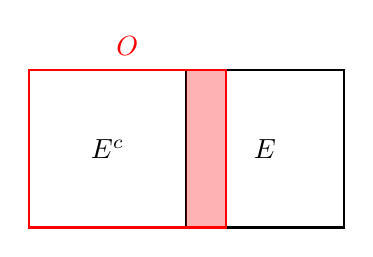
\begin{tikzpicture}
        \draw[thick] (0,0) rectangle (4,2);
        \draw[thick] (2,0) -- (2,2);
        
        \node at (1,1) {$E^c$};
        \fill[red, opacity=0.3] (2,0) rectangle (2.5,2);

        \node at (3,1) {$E$};
        
        % Draw red box O
        \draw[thick, red] (0,0) rectangle (2.5,2);
        \node[red] at (1.25, 2.3) {$O$};
      \end{tikzpicture}
      \caption{The shaded rectangle can be represented as the difference $O \setminus E^c$ or $E \setminus O^c$.} 
    \end{figure}
  \end{solution}

  \begin{exercise}[Royden 2.17]
    Show that a set $E$ is measurable if and only if for each $\epsilon > 0$, there is a closed set $F$ and open set $O$ for which $F \subseteq E \subseteq O$ and $m^{\ast}(O \setminus F) < \epsilon$.
  \end{exercise}
  \begin{solution}
    We prove bidirectionally. 
    \begin{enumerate}
      \item $(\rightarrow)$. If $E$ is measurable, then choose $F, O$ s.t. 
        \begin{equation}
          m^\ast (E \setminus F) < \frac{\epsilon}{2}, m^\ast (O \setminus E) < \frac{\epsilon}{2} \implies m^\ast(O \setminus F) \leq m^\ast (O \setminus E) + m^\ast (E \setminus F) < \epsilon
        \end{equation}
      \item $(\leftarrow)$. 
    \end{enumerate}
  \end{solution}

  \begin{exercise}[Royden 2.18]
    Let $E$ have finite outer measure. Show that there is an $F_{\sigma}$ set $F$ and a $G_{\delta}$ set $G$ such that
    \begin{equation*}
      F \subseteq E \subseteq G \text{ and } m^{\ast}(F) = m^{\ast}(E) = m^{\ast}(G).
    \end{equation*}
  \end{exercise}

  \begin{exercise}[Royden 2.19]
    Let $E$ have finite outer measure. Show that if $E$ is not measurable, then there is an open set $O$ containing $E$ that has finite outer measure and for which
    \begin{equation*}
      m^{\ast}(O \setminus E) > m^{\ast}(O) - m^{\ast}(E).
    \end{equation*}
  \end{exercise} 
  \begin{solution}
    
  \end{solution}

  \begin{exercise}[Royden 2.20]
    (Lebesgue) Let $E$ have finite outer measure. Show that $E$ is measurable if and only if for each open, bounded interval $(a, b)$,
    \begin{equation*}
      b - a = m^{\ast}((a, b) \cap E) + m^{\ast}((a, b) \setminus E).
    \end{equation*}
  \end{exercise}
  \begin{solution}
    Since 
    \begin{equation}
      m^\ast (E) = \inf \bigg\{ \sum_{k=1}^\infty \ell(I_k) \bigg\} < +\infty, 
    \end{equation}
    there exists a covering $\{I_k = (a_k, b_k)\}_k$  of $E$ s.t. 
    \begin{align}
      m^\ast (E) + \epsilon & > \sum_{k=1}^\infty (b_k - a_k) \\ 
                            & = \sum_{k=1}^\infty m^\ast ((a_k, b_k) \cap E) + m^\ast ((a_k, b_k) \setminus E) \\ 
                            & = \sum_{k=1}^\infty m^\ast ((a_k, b_k) \cap E) + \sum_{k=1}^\infty m^\ast ((a_k, b_k) \setminus E) \\ 
                            & \geq m^\ast \bigg( \bigcup_{k=1}^\infty (a_k, b_k) \cap E \bigg) + m^\ast \bigg( \bigcup_{k=1}^\infty (a_k, b_k) \setminus E \bigg) \\ 
                            & = m^\ast (E) + m^\ast (O \setminus E) 
    \end{align}
    which implies $\epsilon > m^\ast (O \setminus E)$, which is equivalent to $E$ being measurable. 
  \end{solution}

  \begin{exercise}[Royden 2.21]
    Use property (ii) of Theorem 11 as the primitive definition of a measurable set and prove that the union of two measurable sets is measurable. Then do the same for property (iv).
  \end{exercise}

  \begin{exercise}[Royden 2.22]
    For any set $A$, define $m^{\ast\ast}(A) \in [0, \infty]$ by
    \begin{equation*}
      m^{\ast\ast}(A) = \inf \{m^{\ast}(O) \mid O \supseteq A, O \text{ open}\}.
    \end{equation*}
    How is this set function $m^{\ast\ast}$ related to outer measure $m^{\ast}$?
  \end{exercise}
  \begin{solution}
    We claim that they are equal. 
    \begin{enumerate}
      \item By monotonicity, $A \subset O \implies m^\ast (A) \leq m^\ast (O)$, and taking the infimum over $O$ gives $m^\ast (A) \leq m^{\ast\ast} (A)$. 
      \item Note that every open set can be represented as a countable pairwise-disjoint union of open intervals, so by countable subadditivity, 
        \begin{equation}
          m^\ast (O) = m^\ast \bigg( \bigcup_{k=1}^\infty (a_k, b_k) \bigg) \leq \sum_{k=1}^\infty \ell ((a_k, b_k)) \implies m^{\ast\ast} (A) \leq m^\ast (A)
        \end{equation}
    \end{enumerate}
  \end{solution}

  \begin{exercise}[Royden 2.23]
    For any set $A$, define $m^{\ast\ast\ast}(A) \in [0, \infty]$ by
    \begin{equation*}
      m^{\ast\ast\ast}(A) = \sup \{m^{\ast}(F) \mid F \subseteq A, F \text{ closed}\}.
    \end{equation*}
    How is this set function $m^{\ast\ast\ast}$ related to outer measure $m^{\ast}$?
  \end{exercise}
  \begin{solution}
    By monotonicity, 
    \begin{equation}
      F \subset A \implies m^\ast (F) \leq m^\ast (A) \implies m^{\ast\ast\ast} (A) \leq m^\ast (A)
    \end{equation}
  \end{solution}

  \begin{exercise}[Royden 2.24]
    Show that if $E_1$ and $E_2$ are measurable, then
    \begin{equation*}
      m(E_1 \cup E_2) + m(E_1 \cap E_2) = m(E_1) + m(E_2).
    \end{equation*}
  \end{exercise}
  \begin{solution}
    We know that $E_1 \cup E_2 = (E_1 \setminus E_2) \cup (E_2 \setminus E_1) \cup (E_1 \cap E_2)$, and so by finite additivity, 
    \begin{equation}
      m(E_1 \cup E_2) = m(E_1 \setminus E_2) + m(E_2 \setminus E_1) + m(E_1 \cap E_2) 
    \end{equation}
    By adding $m(E_1 \cap E_2)$ and grouping, we get 
    \begin{equation}
      m(E_1 \cup E_2) + m(E_1 \cap E_2) = \underbrace{m(E_1 \setminus E_2) + m(E_1 \cap E_2)}_{m(E_1)} + \underbrace{m(E_2 \setminus E_1) + m(E_1 \cap E_2)}_{m(E_2)}
    \end{equation}
  \end{solution}

  \begin{exercise}[Royden 2.25]
    Show that the assumption that $m(B_1) < \infty$ is necessary in part (ii) of the theorem regarding continuity of measure.
  \end{exercise}

  \begin{exercise}[Royden 2.26][ex:royden2.26]
    Let $\{E_k\}_{k=1}^{\infty}$ be a countable disjoint collection of measurable sets. Prove that for any set $A$,
    \begin{equation*}
      m^{\ast}\left(A \cap \bigcup_{k=1}^{\infty} E_k\right) = \sum_{k=1}^{\infty} m^{\ast}(A \cap E_k).
    \end{equation*}
  \end{exercise}
  \begin{solution}
    We know that for all $n \in \mathbb{N}$, 
    \begin{equation}
      \sum_{k=1}^n m^\ast (A \cap E_k) = m^\ast \bigg( A \cap \bigcup_{k=1}^n E_k \bigg) = m^\ast \bigg( \underbrace{\bigcup_{k=1}^n (A \cap E_k)}_{B_n} \bigg)
    \end{equation}
    The $B_n$ are an increasing sequence of sets, so by continuity from below, 
    \begin{equation}
      m \bigg( \bigcup_{n=1}^\infty \bigcup_{k=1}^n (A \cap E_k) \bigg) = \lim_{n \to \infty} m \bigg( \bigcup_{k=1}^n (A \cap E_k) \bigg)
    \end{equation}
    So by taking the limit as $n \to \infty$, 
    \begin{align}
      \sum_{k=1}^\infty m^\ast (A \cap E_k) & = \lim_{n \to \infty} m^\ast \bigg( \bigcup_{k=1}^n (A \cap E_k) \bigg) \\ 
                                            & = m^\ast \bigg( \bigcup_{n=1}^\infty \bigcup_{k=1}^n (A \cap E_k) \bigg) \\ 
                                            & = m^\ast \bigg( \bigcup_{k=1}^\infty (A \cap E_k) \bigg) 
    \end{align}
  \end{solution}
  \begin{solution}
    We know from countable subadditivity that 
    \begin{align}
      m^\ast \bigg( A \cap \bigcup_{k=1}^\infty E_k \bigg) \leq \sum_{k=1}^\infty m^\ast (A \cap E_k) \\ 
    \end{align}
    Now, 
    \begin{equation}
      m^\ast \bigg( A \cap \bigcup_{k=1}^\infty E_k \bigg) \geq m^\ast \bigg( A \cap \bigcup_{k=1}^n E_k \bigg) = \sum_{k=1}^n m^\ast (A \cap E_k)
    \end{equation}
    So by taking $n \to +\infty$, we are done. 
  \end{solution}

  \begin{exercise}[Royden 2.27]
    Let $\mathcal{M}^{\prime}$ be any $\sigma$-algebra of subsets of $\mathbf{R}$ and $m^{\prime}$ a set function on $\mathcal{M}^{\prime}$ which takes values in $[0, \infty]$, is countably additive, and such that $m^{\prime}(\emptyset) = 0$.
    \begin{enumerate}
      \item Show that $m^{\prime}$ is finitely additive, monotone, countably monotone, and possesses the excision property.
      \item Show that $m^{\prime}$ possesses the same continuity properties as Lebesgue measure.
    \end{enumerate}
  \end{exercise}

  \begin{exercise}[Royden 2.28]
    Show that continuity of measure together with finite additivity of measure implies countable additivity of measure.
  \end{exercise}
  \begin{solution}
    This was basically my solution for Exercise \ref{ex:royden2.26}. Let $\{E_k\}_{k=1}^\infty$ be a sequence of sets. Then, $m$ being finitely additive implies that 
    \begin{equation}
      m^\ast \bigg( \bigcup_{k=1}^n E_k \bigg) = \sum_{k=1}^n m(E_k) 
    \end{equation}
    But now define $B_n = \cup_{k=1}^n E_k$, which is increasing, and so by continuity of measure from below, 
    \begin{align}
      m \bigg( \bigcup_{k=1}^\infty E_k \bigg) & = m \bigg( \bigcup_{n=1}^\infty B_n \bigg) \\ 
                                               & = \lim_{n \to \infty} m(B_n) \\ 
                                               & = \lim_{n \to \infty} m \bigg( \bigcup_{k=1}^n E_k \bigg) \\ 
                                               & = \lim_{n \to \infty} \sum_{k=1}^n m(E_k) \\ 
                                               & = \sum_{k=1}^\infty m(E_k)
    \end{align}
  \end{solution}

  \begin{exercise}[Royden 2.29]
    Listed. 
    \begin{enumerate}
      \item Show that rational equivalence defines an equivalence relation on any set.
      \item Explicitly find a choice set for the rational equivalence relation on $\mathbf{Q}$.
      \item Define two numbers to be irrationally equivalent provided their difference is irrational. Is this an equivalence relation on $\mathbf{R}$? Is this an equivalence relation on $\mathbf{Q}$?
    \end{enumerate}
  \end{exercise}

  \begin{exercise}[Royden 2.30]
    Show that any choice set for the rational equivalence relation on a set of positive outer measure must be uncountably infinite.
  \end{exercise}

  \begin{exercise}[Royden 2.31]
    Justify the assertion in the proof of Vitali's Theorem that it suffices to consider the case that $E$ is bounded.
  \end{exercise}

  \begin{exercise}[Royden 2.32]
    Does Lemma \ref{lem:countable-disjoint-translates-0-measure}\footnote{Originally Royden 4th Edition Lemma 11} remain true if $\Lambda$ is allowed to be finite or to be uncountably infinite? Does it remain true if $\Lambda$ is allowed to be unbounded?
  \end{exercise}
  \begin{solution}
    Listed. 
    \begin{enumerate}
      \item Finite? No. Let $E = (0, 1)$ and $\Lambda = \{0, 1, 2\}$. Therefore, the infinite part is essential since it makes things harder to overlap. 
      \item Uncountably infinite? Yes, since we can just find a countably infinite subcollection from it. 
      \item $\Lambda$ unbounded? No. Let $E = (0, 1)$ and $\Lambda = \mathbb{Z}$. Then, $\{E + z\}_{z \in \mathbb{Z}}$ are disjoint but $m(E) = 1$. If it was unbounded, then we can just give as much space for $E + \lambda$ to roam around.  
    \end{enumerate}
  \end{solution}

  \begin{exercise}[Royden 2.33]
    Let $E$ be a nonmeasurable set of finite outer measure. Show that there is a $G_{\delta}$ set $G$ that contains $E$ for which
    \begin{equation*}
      m^{\ast}(E) = m^{\ast}(G), \text{ while } m^{\ast}(G \setminus E) > 0.
    \end{equation*}
  \end{exercise}
  \begin{solution}
    Note from Exercise \ref{ex:royden2.7} that we can outer-approximate \textit{any} set with a $G_\delta$-set. Therefore, choose such a set $G \supset E$ which satisfies 
    \begin{equation}
      m^\ast (G) - m^\ast (E) = 0 
    \end{equation}
    If $E$ was measurable, then by excision property, $m^\ast(G \setminus E) = 0$, but $E$ is not measurable, so we must have $m^\ast(G \setminus E) > 0$. 
  \end{solution}

  \begin{exercise}[Royden 2.34]
    Show that there is a continuous, strictly increasing function on the interval $[0, 1]$ that maps a set of positive measure onto a set of measure zero.
  \end{exercise}

  \begin{exercise}[Royden 2.35]
    Let $f$ be an increasing function on the open interval $I$. For $x_0 \in I$ show that $f$ is continuous at $x_0$ if and only if there are sequences $\{a_n\}$ and $\{b_n\}$ in $I$ such that for each $n$, $a_n < x_0 < b_n$, and $\lim_{n \to \infty}[f(b_n) - f(a_n)] = 0$.
  \end{exercise}

  \begin{exercise}[Royden 2.36]
    Show that if $f$ is any increasing function on $[0, 1]$ that agrees with the Cantor-Lebesgue function $\varphi$ on the complement of the Cantor set, then $f = \varphi$ on all of $[0, 1]$.
  \end{exercise}

  \begin{exercise}[Royden 2.37]
    Let $f$ be a continuous function defined on $E$. Is it true that $f^{-1}(A)$ is always measurable if $A$ is measurable?
  \end{exercise}

  \begin{exercise}[Royden 2.38][ex:royden2.38]
    Let the function $f : [a, b] \to \mathbf{R}$ be Lipschitz, that is, there is a constant $c \geq 0$ such that for all $u, v \in [a, b]$, $|f(u) - f(v)| \leq c|u - v|$. Show that $f$ maps a set of measure zero onto a set of measure zero. Show that $f$ maps an $F_{\sigma}$ set onto an $F_{\sigma}$ set. Conclude that $f$ maps a measurable set to a measurable set.
  \end{exercise}

  \begin{exercise}[Royden 2.39]
    Let $F$ be the subset of $[0, 1]$ constructed in the same manner as the Cantor set except that each of the intervals removed at the $n$th deletion stage has length $\alpha 3^{-n}$ with $0 < \alpha < 1$. Show that $F$ is a closed set, $[0, 1] \setminus F$ dense in $[0, 1]$, and $m(F) = 1 - \alpha$. Such a set $F$ is called a generalized Cantor set.
  \end{exercise}

  \begin{exercise}[Royden 2.40]
    Show that there is an open set of real numbers that, contrary to intuition, has a boundary of positive measure. (Hint: Consider the complement of the generalized Cantor set of the preceding problem.)
  \end{exercise}

  \begin{exercise}[Royden 2.41]
    A nonempty subset $X$ of $\mathbf{R}$ is called perfect provided it is closed and each neighborhood of any point in $X$ contains infinitely many points of $X$. Show that the Cantor set is perfect. (Hint: The endpoints of all of the subintervals occurring in the Cantor construction belong to $C$.)
  \end{exercise}

  \begin{exercise}[Royden 2.42]
    Prove that every perfect subset $X$ of $\mathbf{R}$ is uncountable. (Hint: If $X$ is countable, construct a descending sequence of bounded, closed subsets of $X$ whose intersection is empty.)
  \end{exercise}

  \begin{exercise}[Royden 2.43]
    Use the preceding two problems to provide another proof of the uncountability of the Cantor set.
  \end{exercise}

  \begin{exercise}[Royden 2.44]
    A subset $A$ of $\mathbf{R}$ is said to be \emph{nowhere dense in} $\mathbf{R}$ provided that for every open set $O$ has an open subset that is disjoint from $A$. Show that the Cantor set is nowhere dense in $\mathbf{R}$.
  \end{exercise}

  \begin{exercise}[Royden 2.45]
    Show that a strictly increasing function that is defined on an interval has a continuous inverse.
  \end{exercise}

  \begin{exercise}[Royden 2.46]
    Let $f$ be a continuous function and $B$ be a Borel set. Show that $f^{-1}(B)$ is a Borel set. (Hint: The collection of sets $E$ for which $f^{-1}(E)$ is Borel is a $\sigma$-algebra containing the open sets.)
  \end{exercise}

  \begin{exercise}[Royden 2.47]
    Use the preceding two problems to show that a continuous strictly increasing function that is defined on an interval maps Borel sets to Borel sets.
  \end{exercise}

  \begin{exercise}[Math 631 Fall 2025, Midterm Exercise 1]
    Define a set $E \subset [0, 1]$ to be all points such that in their decimal expansion the 10th digit (corresponding to $10^{-10}$ value) is equal to 4, and the 100th digit is equal to 5. Show that $E$ is measurable and find $m(E)$.
  \end{exercise}
  \begin{solution}
    There is just a finite set of real numbers where the ambiguity of the decimal expansion affects the definition of set $E$: for example, $0.0000000004000... = 0.00000000039999...$ - but finite number of points does not affect that measurability or Lebesgue measure of a set. We can adopt the convention that whenever we can use 4 on 10th place and 5 on the 100th place, we do. With this convention, the set of points with 4 on the 10th decimal place is a set of $10^9$ disjoint closed intervals $I_k$ of size $10^{-10}$. These intervals correspond to the $10^9$ choices of all possible digits in the larger position values. We further insist that 5 stands on the 100th place, then in each $I_k$ there are $10^{89}$ closed intervals of size $10^{-100}$ where this is true. The number $10^{89}$ corresponds to all possible choices of digits at 89 positions from 11th to 99th. So, there is a total of
    \begin{equation}
      10^9 \times 10^{89} = 10^{98}
    \end{equation}
    disjoint intervals of size $10^{-100}$. This set is measurable as a finite union of intervals. The Lebesgue measure of such set is 0.01 by additivity of the Lebesgue measure.
  \end{solution}

  \begin{exercise}[Math 631 Fall 2025, Final Exam Exercise 3]
    Let $E_{k}\subset(0,1)$ be measurable sets. Is it true that there exists a subsequence $E_{k_{j}}$ such that $m(\cap_{j}E_{k_{j}})>0$ if (a) $\limsup m(E_{k})=1$, (b) $\liminf m(E_{k})>3/4$?
  \end{exercise}
  \begin{solution}
    (a) Yes. Choose a subsequence $k_{j}$ such that $\sum_{j=1}^{\infty}(1-m(E_{k_{j}}))<1$. This can be achieved, for example, if we require that $1-m(E_{k_{j}})<2^{-j}$. This is equivalent to
    \begin{equation}
      \sum_{j=1}^{\infty}m(E_{k_{j}}^{c})<1.
    \end{equation}
    This implies by countable subadditivity that $m(\cup_{j=1}^{\infty}E_{k_{j}}^{c})<1$, and since $\cap_{j}E_{k_{j}}=(\cup_{j=1}^{\infty}E_{k_{j}}^{c})^{c}$, we get $m(\cap_{j}E_{k_{j}})>0$.

    (b) No. Let $E_{k}$ be all numbers without digits 1 and 2 at the $k$th position in their decimal expansion. Then $m(E_{k})=4/5$ for every $k$. On the other hand, for any $k_{j}$,
    \begin{equation}
      m(\cap_{j=1}^{J}E_{k_{j}})=(4/5)^{J}\rightarrow0
    \end{equation}
    as $J\rightarrow\infty$.
  \end{solution}

